\chapter{Morphophonology}\label{section:morphophono}

In terms of the interaction between morphology and phonology, we discuss mor\-phol\-o\-gi\-cal\-ly-in\-duced phonological processes (\S\ref{section:morphophono:morphophono}),  phonologically-con\-di\-tioned allomorphy (\S\ref{section:morphophono:allomorphy}), and a phonosyntactic process that references both phonology and syntax (\S\ref{section:morphophono:auxiliary}). 

\section{Morphophonological alternations}\label{section:morphophono:morphophono}
Besides general phonology, Armenian dialects show various morphophonological rules which operate at morpheme boundaries. This includes root-initial glide insertion (\S\ref{section:morphophono:morphophono:root initial glide}), vowel hiatus repair under suffixation/cliticization (\S\ref{section:morphophono:morphophono:vowel hiatus}), and high vowel   reduction under suffixation (\S\ref{section:morphophono:morphophono:vowel reduction}).  

In general,   morphophonological processes that are attested in {\seaSEA}  are also attested in {\iaIA}. But in the judgments of KM, ``phonological changes at morpheme boundaries are becoming simpler in {\iaIA}.'' This ``simplicity'' suggests that such processes apply less often in {\iaIA} than in {\seaSEA}. For an overview of such morphophonological processes in {\seaSE} and {\swaWA}, see \citet[\S1]{Vaux-1998-ArmenianPhono} and \citet[\S2]{Dolatian-2020-Diss}.


\subsection{Root-initial glide insertion }\label{section:morphophono:morphophono:root initial glide}
Armenian is primarily suffixing, and there are few morphophonological rules that are sensitive to prefix boundaries. The most noticeable process is root-initial  “diphthongization” or glide insertion.

The Classical Armenian grapheme \armenian{ե} 
was a mid vowel \textit{{e}} \citep{Macak-2017-PhonoClassicalArmenian}. In the diachronic development from Classical Armenian to modern Armenian, this grapheme later underwent root-initial glide insertion \citep{weitenberg-2008-diphthongizationInitialEInitialYArmenian}. For example  in {\seaSEA}, the word-initial pronunciation of this grapheme is [{{je}}] (Table \ref{tab:MorphoPhono:GlideInsertion}). In {\seaSE}, the glide is prescriptively supposed to delete   after inflectional prefixes like the synthetic future \textit{{k-}} and negative \textit{{t͡ʃʰ-}}, but the retention of the glide has become more common in {\seaCEA} \citep[15]{DumTragut-2009-ArmenianReferenceGrammar}. For {\iaIA}, the retention seems obligatory based on our elicitations, at least for NK and her family. These prefixes trigger schwa epenthesis before a consonant.

\begin{table}[p]
	\caption{Root-initial glide insertion from NK}\label{tab:MorphoPhono:GlideInsertion}
	\resizebox{\textwidth}{!}{%
		\begin{tabular}{lllll}
			\lsptoprule
			&{\seaAbbre} &{\iaAbbre} &&\\\midrule 
			\armenian{երգել} & {jeɾkʰ-e-l}   & {jeɻkʰ-e-l}&$\sqrt{~}$-{\thgloss}-{\infgloss}  &`to sing'\\
			\armenian{երգեմ} & {jeɾkʰ-e-m}   & {jeɻkʰ-e-m}&$\sqrt{~}$-{\thgloss}-1{\sg}  &`I sing ({\subj})'\\
			\armenian{կերգեմ}  	%		\armenian{կ՚երգեմ} 
			& {k-eɾkʰ-e-m}   & {} &{\fut}-$\sqrt{~}$-{\thgloss}-1{\sg} &`I {will} sing' \\
			& {kə-jeɾkʰ-e-m}   & {kə-jeɻkʰ-e-m} & & \\
			\armenian{չերգեմ} & {t͡ʃʰ-eɾkʰ-e-m}   & {} &{\neggloss}-$\sqrt{~}$-{\thgloss}-1{\sg} &`I don't sing ({\subj})'\\
			& {t͡ʃʰə-jeɾkʰ-e-m}   & {t͡ʃʰə-jeɻkʰ-e-m}  &&\\
			\lspbottomrule
		\end{tabular}%
		}
\end{table}


However, there are some lexemes which   have the initial <\armenian{\#{ե}}> 
[{\#je}] in {\seaSEA}, but where the glide is lost in {\iaIA} (\tabref{tab:MorphoPhono:GlideLoss}).  For some of these lexemes, {\seaCEA} also has dialectal forms without the glide.  The loss of the glide in {\iaIA} is likely a sporadic and idiosyncratic diachronic process because the relevant lexemes are high-frequency words, and  oftentimes function   words.\footnote{For the word `yesterday' in {\iaIA}, NK and her family tend to say this word as [eɻeɡ], while KM and AS report [eɻek].}

\begin{table}[p]
\caption{Loss of initial glides in {\iaIA}}\label{tab:MorphoPhono:GlideLoss}
	\begin{tabular}{llll}
		\lsptoprule 
		& {\seaAbbre} & {\iaAbbre} &\\\midrule
		\armenian{երեկ} & {jeɾek $\sim$ eɾek}  & {eɻek}     & `yesterday'\\
		\armenian{երթալ} & {jeɾtʰɑl $\sim$ eɾtʰɑl $\sim$ etʰɑl}   & {eɻtʰɒl $\sim$ etʰɒl}& `to go'\\
		\armenian{երկու} & {jeɾku $\sim$ eɾku}  & {eɻku} &`two'\\
		\armenian{եփել} & {jepʰel $\sim$ epʰel}  & {epʰel} &`to cook'\\
		\armenian{ելնել} & {jelnel $\sim$ elnel}  & {elnel} &`to rise' ({\seaAbbre});\\
		& & &  `to be' ({\iaAbbre})\\
		\armenian{եկել} & {jekel $\sim$ ekel}  & {ekel $\sim$ ekeɻ} &`to  come ({\rptcp})'
		\\ \lspbottomrule
	\end{tabular}
\end{table}

\begin{table}[p]
\caption{Maintaining  initial [v] in {\iaIA}}\label{tab:MorphoPhono:Process:Vpreserve}
%{%\resizebox{.9\textwidth}{!}{%
	\begin{tabular}{lllll}
		\lsptoprule
		& {\seaAbbre} & {\seaCEAAbbre} & {\iaAbbre} &\\\midrule
		\armenian{ոսպ}
		& {vosp}  						& {vosp}  & {vosp}     & `lentil'\\
		\armenian{որոշել}& {voɾoʃel}						& {voɾoʃel}   & {voɻoʃel}& `to decide' \\
		\armenian{կորոշեմ}& {k-oɾoʃem}   & kə-voɾoʃem & {kə-voɻoʃem}& `I {will} decide' \\
		\lspbottomrule
	\end{tabular}
\end{table}
		
		The words that show this glide-to-zero change  are all polysyllabic.  We have found monosyllabic words that have an invariant glide, such as [jeɻpʰ] `when' \armenian{երբ} and [jeɻkʰ] `song' \armenian{երգ}. But we have not been able find monosyllabic roots where the glide is deleted. It is possible that glide deletion is only allowed in polysyllabic roots. 
		
		When   glide insertion applies word-initially, the orthographic convention is to write the word with an initial letter <\armenian{ե}>. When the glide is absent, the convention is to use the letter <\armenian{է}>. For example, the word `to cook' with a glide [{jepʰel}] is spelled \armenian{եփել},  while the glide-less form [{epʰel}] is spelled \armenian{էփել}.  
		
		A related process is how the  letters <\armenian{ո, օ}> are pronounced [vo, o] root-initially, but both as [o] root-medially (Table \ref{tab:MorphoPhono:Process:Vpreserve}). For the letter \armenian{ո}, it seems that this letter is  always pronounced as [vo] word-initially in both monosyllables  and polysyllables.  In {\seaSEA}, a root-initial and word-medial  [vo] changes to   [o]    in  prefixation, but {\seaCEA} and {\iaIA} prefer keeping this root-initial [vo] as [vo]  \citep[16]{DumTragut-2009-ArmenianReferenceGrammar}.  More data is needed to verify these tendencies.  
			
		
		\subsection{Vowel hiatus repair}\label{section:morphophono:morphophono:vowel hiatus}
  
		Within the word, vowel-vowel sequences (vowel hiatus) are typically repaired, such as via [{j}] epenthesis or by changing [{u}] to [{v}]. {\iaIA} seems to utilize all the vowel hiatus repair rules that are used by {\seaSE}. {\iaIA} is however innovative in that it can also epenthesize a [{w}] glide.
		
		Across the stem-inflection boundary in {\seaSEA}, pre-vo\-cal\-ic /{i}/ tends to delete  (\ref{example glide epenth and fortification}a) while pre-vocalic /{u}/ tends to de-vocalize or change to [{v}] (\ref{example glide epenth and fortification}b). Less common strategies are to epenthesize a glide [{j}] in these contexts.   The following data uses the instrumental suffix /-ov/. 
		
		
		\begin{exe}
			\ex \textit{/{u}/ devocalization and /{i}/ deletion in vowel hiatus}\label{example glide epenth and fortification}
			
			
			\begin{tabular}{lllll}
				& {\seaAbbre} & {\iaAbbre} & & \\
				
				a. & 	{ɑjɡi}&{ɒjɡi} &`garden' & \armenian{այգի}
				\\
				&	{ɑjɡ-ov}&{ɒjɡ-ov} &`garden-{\ins}'& \armenian{այգով}
				\\
				& 		{ɑjɡi-jov}&{ɒjɡi-jov} && \armenian{այգիով}
				\\
				b. & 			{lezu}&   {lezu} &`tongue'  & \armenian{լեզու}\\
				& {lezv-ov}&{lezv-ov} &`tongue-{\ins}'  & \armenian{լեզվով} (Reformed) 
				\\
				& &  & & \armenian{լեզուով} (Classical)
				\\
				&
				{lezu-jov}&{lezu-jov} && \armenian{լեզուով}
			\end{tabular}
		\end{exe}

  
		In KM’s judgments for pre-vocalic /{u}/, {\iaIA} utilizes /u/-de\-vo\-cal\-i\-za\-tion  and /{i}/-deletion less often than {\seaSE}, while {\iaIA}  utilizes /{j}/-insertion more often than {\seaSE}. 
		
		\begin{sloppypar}
		Unlike {\seaSE}, {\iaIA}   utilizes /w/-insertion to repair vowel hiatus in a cliticized /u=V/ sequence (\ref{sent:MorphPhono:Process:Hiatus:w}). Inserting a glide /w/  is obligatory if the /{u}/ is part of the future converb. The second vowel is part of the inflected auxiliary, and the vowel can be /{e, ɒ, i/}. We provide stress markings to reinforce the fact that the final vowel is a clitic. We do not provide a finer segmentation for the auxiliary.
		\end{sloppypar}
		
		\begin{exe}
			\ex \textit{/w/-insertion for cliticized future converbs}\label{sent:MorphPhono:Process:Hiatus:w}
			
			\begin{tabular}{lll}
				
				{/jeɻkʰ-e-l-u=em/}  &
				{jeɻ.kʰe.ˈ\textbf{lu}.wem}  & `I will sing'
				\\
				& & \armenian{երգելու եմ}\\
				/{jeɻkʰ-e-l-u=iɻ}/ &
				{jeɻ.kʰe.ˈ\textbf{lu}.wiɻ} &`you were going to sing'
				\\
				& & \armenian{երգելու իր}\\
				/{jeɻkʰ-e-l-u=ɒ}/&
				{jeɻ.kʰe.ˈ\textbf{lu}.wɒ} & `he will sing'
				\\
				$\sqrt{~}$-{\thgloss}-{\infgloss}-{\futcvb}={\auxgloss}
				& & \armenian{երգելու ա}\\
				
				
			\end{tabular}
		\end{exe}
		
		
		Rule \ref{rule:MorphPhono:Process:Hiatus:w} is a rule for vowel hiatus repair in the future converb.
		
		\begin{newruleblock}[rule:MorphPhono:Process:Hiatus:w]{Morpheme-specific rule of {w}-\textit{epenthesis}}
			
				\begin{tabular}{llll}
					$\emptyset$ & $\rightarrow$ & [{w}] & / u\textsubscript{1} \_ V\textsubscript{2} 
					\\
					&&&where /{u}\textsubscript{1}/ is the future converb suffix, 
					\\
					& & & and /V\textsubscript{2}/ is the auxiliary
			\end{tabular}
			
		\end{newruleblock} 
		
		
		
		Insertion of /w/  is also attested outside of the future converb (\ref{sent:MorphPhono:Process:Hiatus:wNotFut}). When  an enclitic is attached to a /u/-final noun, the typical vowel hiatus repair rule is to insert [{j}]. But NK and AS  report  that /w/-insertion is also possible.
		
		\begin{exe}
			\ex \textit{/w/-insertion outside of the future converb}\label{sent:MorphPhono:Process:Hiatus:wNotFut}
			
			\begin{tabular}{ll}
				a. 	& /{kɒtu=e-m}/   \\
				& 		{kɒ.ˈ\textbf{tu}.jem} \textit{or}
				{kɒ.ˈ\textbf{tu}.wem}
				\\
				&	cat={\auxgloss}-1{\sg}
				\\
				& 			`I am a cat.'
				\\
				&\armenian{ Կատու եմ։}
				\\
				b. 	& /{kɒtu=el=e-m}/   \\
				& 		{kɒ.ˈ\textbf{tu}.je.lem} \textit{or}
				{kɒ.ˈ\textbf{tu}.we.lem}
				\\
				&	cat=also={\auxgloss}-1{\sg}
				\\
				& 			`I am also a cat.'
				\\
				&\armenian{Կատու էլ եմ։}
			\end{tabular}
		\end{exe}
		
		It is possible that {\iaIA} innovated a rule of /w/-insertion because of contact with Persian. Persian allows various types of vowel hiatus repair rules  (\citealt[3]{ariyaeeJurgec-2021-variableHiatusPersianAffectedSuffixLength}). One such rule   inserts the glide [{w}] after a back vowel /{u}/ \citep[20]{dehghan-2012-shortAnalysisInsertionPersian}.
		
		
		
		\subsection{Destressed high vowel reduction}\label{section:morphophono:morphophono:vowel reduction}
		
		Armenian utilizes a process of destressed high vowel reduction (\citealt{Vaux-1998-ArmenianPhono,Khanjian-2009-StressShift,Dolatian-2020-Diss,Dolatian-2020-NLLTArmenianReduction}). When a root undergoes suffixation, regular final stress typically shifts to the suffix (Table \ref{tab:MorphPhono:Process:Destressed:Basic}). In {\seaSE} and {\iaIA}, destressed high vowels from the root reduce before derivational suffixes, but generally not before consonant-initial inflectional suffixes. Some words exceptionally reduce before the consonant-initial \textit{-neɻ}.\footnote{See footnote \ref{footnote utjun} in \chapref{section phono} on the difference in the pronunciation of the suffix   /-utʰjun/.  }
		
		\begin{table}
			\caption{Destressed high vowel reduction}\label{tab:MorphPhono:Process:Destressed:Basic}
			\begin{tabular}{llll}
				\lsptoprule
				{\seaAbbre} & {\iaAbbre} & &\\\midrule
				ɑmuˈ\textbf{sin}  & ɒmuˈ\textbf{sin} & `husband' & \armenian{ամուսին}\\
				ɑmu\textbf{sn}-uˈtʰjun & ɒmu\textbf{sn}-uˈt͡ʃʰun & `marriage' & \armenian{ամուսնութիւն}\\
				ɑmu\textbf{sin}-ˈneɾ  & ɒmu\textbf{sin}-ˈneɻ & `husbands' & \armenian{ամուսիններ}\\
				\midrule
				ˈsk\textbf{i}zb  & ˈsk\textbf{i}zb  & `beginning' & \armenian{սկիզբ}\\
				sk\textbf{i}zb-ˈneɾ &  sk\textbf{i}zb-ˈneɻ & `beginnings' & \armenian{սկիզբներ}\\
				sk\textbf{ə}zb-ˈneɾ &  sk\textbf{ə}zb-ˈneɻ & `beginnings' & \armenian{սկզբներ}\\ 
				\lspbottomrule
			\end{tabular}
		\end{table}
		
		Before vowel-initial inflectional suffixes, the tendency in {\seaSEA} is for reduction to apply (\ref{tab:MorphPhono:Process:Destressed:Infl}). For {\iaIA}, KM feels that reduction applies less often in this context    than in {\seaSE}. 
		
		\begin{exe}
			\ex   \textit{Variation in vowel reduction before V-initial inflection}\label{tab:MorphPhono:Process:Destressed:Infl}
			
			\begin{tabular}{ ll ll }
				a. & 
				{kɒmˈ\textbf{u}ɻd͡ʒ}& `bridge' &  \armenian{կամուրջ}
				\\
				& 	{kɒm\textbf{u}ɻˈd͡ʒ-it͡sʰ}&`bridge-{\abl}' &  \armenian{կամուրջից}
				\\
				& 	{kɒm\textbf{ə}ɻˈd͡ʒ-it͡sʰ}&  &  \armenian{կամրջից}
				\\
				b. &  	{jeɻˈk\textbf{i}ɻ}  & `world' & \armenian{երկիր}
				\\
				& 
				{jeɻk\textbf{i}ˈɻ-um}  & `world-{\locgloss}' & \armenian{երկիրում}
				\\
				&
				{jeɻ\textbf{kˈɻ}-um }  & & \armenian{երկրում}
				\\
				c. 			&
				{ˈt\textbf{u}n}  & `house' & \armenian{տուն}\\
				
				&
				{t\textbf{u}ˈn-um}  & `house-{\locgloss}'  & \armenian{տունում}
				
				\\
				&
				{t\textbf{ə}ˈn-um }  & & \armenian{տնում}  \\
				
			\end{tabular}
			
		\end{exe}
		
		Before vowel-initial inflectional suffixes, there is widespread cross-dialectal and   lexical variation in the application of high vowel reduction \citep{Gharagulyan-1974-BookArmenianOrthoepy,Margaryan-1997-ArmenianPhonology}. For an overview, see \citet[41ff]{DumTragut-2009-ArmenianReferenceGrammar} and  \citet[\S2.7]{Dolatian-2020-NLLTArmenianReduction}.
		
		\section{Phonologically-conditioned allomorphy}\label{section:morphophono:allomorphy}
		This section   presents some examples of phonologically-conditioned allomorphy in {\iaIA}. These include syllable-counting allomorphy of the plural suffix  (\S\ref{section:morphophono:allomorphy: syll}), schwa-zero and schwa-nasal alternations for the possessive and definite suffixes (\S\ref{section:morphophono:allomorphy: det}),  and variable voicing assimilation in the synthetic future prefix  (\S\ref{section:morphophono:allomorphy: cond}). 
		
		\subsection{Syllable-counting allomorphy of the plural suffix}\label{section:morphophono:allomorphy: syll}
		
		
		For the plural, the regular suffix is \textit{{-eɻ}} for monosyllabic bases, and \textit{{-neɻ}} for polysyllabic bases \citep{Vaux-2003-Syllabification,dolatian-2020-MorhpologyRoleCompounds}. This is a relatively straightforward case of syllable-counting allomorphy, as a form of phonologically-conditioned allomorphy (Table \ref{tab:MorphPhono:Process:Allom:Pl}). 
		
		
		\begin{table}
			\caption{Distribution of regular plural suffixes}\label{tab:MorphPhono:Process:Allom:Pl}
			\begin{tabular}{llllll}
				\lsptoprule
				\multicolumn{3}{c}{Monosyllabic} & \multicolumn{3}{c}{Polysyllabic}\\\cmidrule(lr){1-3}\cmidrule(lr){4-6}
				{bɒr} & `word'&\armenian{բառ}& {senjɒk} & `room'&\armenian{սենեակ}\\
				{bɒr-eɻ} & `words'&\armenian{բառեր}& {senjɒk-neɻ} & `rooms'&\armenian{սենեակներ}\\
				\lspbottomrule
			\end{tabular}
		\end{table}
		
		Words that have only one syllable and the appendix \textit{-kʰ} count as monosyllabic for plural-counting (Table \ref{tab:MorphPhono:Process:Allom:PlFunny}).\footnote{Compounds have complicated rules for plural allomorphy in Armenian \citep[21]{Vaux-1998-ArmenianPhono}. For discussion, see \citet{dolatian-2020-MorhpologyRoleCompounds,Dolatian-2022-VariationBracketingParadoxArmenianCompound}.} Words with an initial appendix /s/  +    a syllable are treated as polysyllabic. 
  
  
		
		\begin{table}
			\caption{Pluralization of exceptional syllable structures}\label{tab:MorphPhono:Process:Allom:PlFunny}
			\begin{tabular}{llllll}
				\lsptoprule 				
				\multicolumn{3}{c}{syllable + /-kʰ/} & \multicolumn{3}{c}{/s/ + syllable}\\\cmidrule(lr){1-3}\cmidrule(lr){4-6}
				pɒɻtkʰ  & `debt' & \armenian{պարտք} & 		skizb  & `beginning' & \armenian{սկիզբ}\\
				pɒɻtkʰ-eɻ & `debts'  & \armenian{պարտքեր}& 		skizb-neɻ  & `beginnings' & \armenian{սկիզբներ}\\
				& &   & 	  	  skəzb-neɻ  & & \armenian{սկզբներ}\\
% % 				\midrule
				kuɻt͡skʰ  & `breast' & \armenian{կուրծք} & &&\\
				kuɻt͡skʰ-eɻ & `breasts'  & \armenian{կուրծքեր}& & & 
\\\cmidrule(lr){1-6}

\multicolumn{6}{c}{Syllable +  [CəC]}    \\ \cmidrule(lr){1-6}
vɒɡəɻ & `tiger' & \armenian{վագր} 
& pʰokʰəɻ & `small' & \armenian{փոքր} 
\\
vɒɡɻ-eɻ & `tigers'  & \armenian{վագրեր} 
& pʰokʰɻ-eɻ & `small ones' & \armenian{փոքրեր} 
\\
vɒɡəɻ-neɻ &   & \armenian{վագրներ} 
& pʰokʰəɻ-neɻ &      & \armenian{փոքրներ} 
\\

\lspbottomrule
			\end{tabular}
		\end{table}
		
		Bisyllabic words that end in a [CəC] sequence have an epenthetic schwa, such as [vɒɡəɻ]   `tiger' from /vɒɡɻ/ \citep{Vaux-2003-Syllabification,Dolatian-prep-Schwa}. For modern {\seaSEA}, the plural ignores this schwa and the word is treated as monosyllabic with [-eɾ], such `tigers' [vɑɡɾ-eɾ] \citep[65]{DumTragut-2009-ArmenianReferenceGrammar}. But in older or colloquial registers, the form [-neɾ] is attested like [vɑɡəɾ-neɾ] \citep[217]{Sargsyan-1987-DoubletsNouns}. For {\iaIA}, Anooshik Melikian (AM) reports that the modern community likewise almost always uses [-eɻ], while older members (such as her grandfather) would  use [-neɻ]. 
		
		\subsection{Schwa alternations in the determiner slot}\label{section:morphophono:allomorphy: det}\largerpage
		
		In nominal inflection, the determiner slot is occupied by either a possessive suffix or a definite suffix. Both types of suffixes  display allomorphy conditioned by consonant- vs. vowel-final stems. The definite suffix likewise displays outwardly-conditioned allomorphy to subsequent vowels.
		
		
		The possessive suffixes are \textit{-s}, \textit{-t} for vowel-final bases. A schwa is epenthesized after consonant-final bases (Table \ref{poss allomorphy}). The epenthetic schwa is maintained between a C-final base and a V-initial clitic.
		
		
		
		
		
		
		
		\begin{table}
			\caption{Allomorphy in possessive marking}
			\label{poss allomorphy}
			\begin{tabular}{llll}
				\lsptoprule
				\multicolumn{4}{l}{\textit{No epenthesis after V-final base}}\\
				
				{kɒtu} & &`cat' & \armenian{կատու}\\
				{kɒtu-s} & cat-{\possFsg}&`my cat' & \armenian{կատուս}\\
				{kɒtu-s=el} & cat-{\possFsg}=also&`also my cat' & \armenian{կատուս էլ}\\
				{kɒtu-t} & cat-{\possSsg}&`your cat' & \armenian{կատուդ}\\
				{kɒtu-t=el} & cat-{\possSsg}=also&`also your cat' & \armenian{կատուդ էլ}\\\addlinespace
				\multicolumn{4}{l}{\textit{Schwa epenthesis after C-final base}}\\
				{ɡumɒɻ} & &`amount' & \armenian{գումար}\\
				{ɡumɒɻ-əs} &amount-{\possFsg} &`my amount' & \armenian{գումարս}\\
				{ɡumɒɻ-əs=el} &amount-{\possFsg}=also &`also my amount' & \armenian{գումարս էլ}\\
				{ɡumɒɻ-ət} &amount-{\possSsg} &`your amount' & \armenian{գումարդ}\\
				{ɡumɒɻ-ət=el} &amount-{\possSsg}=also &`also your amount' & \armenian{գումարդ էլ}\\
				\lspbottomrule
			\end{tabular}
			
		\end{table}
		
		
		
The definite suffix has three allomorphs: \textit{{-ə, -n, -ən}} (Table \ref{tab:MorphoPhono:Allo:Def}). The choice of suffix is conditioned by the preceding segment and the following segment.  		When there is no following segment, the suffix is \textit{{-n}} after vowel-final bases, but \textit{{-ə}} after consonant-final stems. 
		
		\begin{table}
			\caption{Forms of the definite suffix in {\seaSE} and {\iaIA}}
			\label{tab:MorphoPhono:Allo:Def}
			\resizebox{\textwidth}{!}{%
				\begin{tabular}{llllll}
					\lsptoprule
					& {\seaAbbre} & {\iaAbbre} && & \\\midrule
					&{kɑˈtu}&{kɒˈtu} & &`cat' & \armenian{կատու}\\
					V\_ & {kɑˈtu-\textbf{n}}& {kɒˈtu-\textbf{n}} &cat-{\defgloss} &`the cat'& \armenian{կատուն}\\
					V\_V & {kɑˈtu-\textbf{n}=el}& {kɒˈtu-\textbf{n}=el} &cat-{\defgloss}=also  &`also the cat'& \armenian{կատուն էլ}\\
					& {kɑˈtu-\textbf{n}=e}& {kɒˈtu-\textbf{n}=ɒ} &cat-{\defgloss}={\auxgloss}  &`is the cat'& \armenian{կատուն է/ա}\\
					\midrule 
					&{ɡuˈmɑɾ}&{ɡuˈmɒɻ}&  &`amount'& \armenian{գումար}\\
					C\_ &{ɡuˈmɑɾ-\textbf{ə}}&{ɡuˈmɒɻ-\textbf{ə}} &amount-{\defgloss} &`the amount'			& \armenian{գումարը}\\
					C\_V &{ɡuˈmɑɾ-\textbf{n}=el}&{ɡuˈmɒɻ-\textbf{ən}=el} & amount-{\defgloss}=also &`also the amount'			& \armenian{գումարն էլ}\\ 
					&{ɡuˈmɑɾ-\textbf{n}=e}&{ɡuˈmɒɻ-\textbf{ən}=ɒ} & amount-{\defgloss}={\auxgloss} &`is the amount'			& \armenian{գումարն է/ա}\\ 
					\lspbottomrule
				\end{tabular}
			}
		\end{table}
		
		The lects differ when the definite suffix is between a C-final base and  V-initial clitic (\ref{tab:MorphoPhono:Allo:DefClitic}). In this context, {\seaSEA} uses the \textit{{-n}} form of the definite.  In {\iaIA}, the form is \textit{{-ən}}. More examples are shown below.\pagebreak
		
		\begin{exe}
			\ex \textit{Other examples of the /{-ən}/ form before clitics in {\iaIA}}\label{tab:MorphoPhono:Allo:DefClitic}
			
			\begin{tabular}{ llll}
				{ˈmɒɻtʰ-\textbf{ən}=ɒ}  & man-{\defgloss}={\auxgloss} & `(he) is the man'&\armenian{մարդն ա}
				\\
				{ˈiŋkʰ-\textbf{ən}=ɒ}  & he-{\defgloss}={\auxgloss} &`it is he' 
				& \armenian{ինքն ա}\\ 
				{dɒˈnɒk-\textbf{ən}=ɒ}  & knife-{\defgloss}={\auxgloss} &`(it) is the knife' &\armenian{դանակն ա}
				\\
			\end{tabular}
		\end{exe}
		
{\iaIA} also uses the     \textit{{-ən}} form   between a C-final word and a V-initial word (\ref{tab:MorphoPhono:Allo:DefWord}).
		
		\begin{exe}
			\ex \textit{Use of -ən before a V-initial word} \label{tab:MorphoPhono:Allo:DefWord}
			
			\begin{xlist}
				\ex \gll 	 ˈiŋkʰ-\textbf{ən} iɻ 
				\\
				him-{\defgloss} he.{\gen} 
				\\ \trans  `himself' \hfill (KM)  \\   \armenian{ինքն իր}
				\ex \gll 			{mɒɻtʰ-\textbf{ən}}   {ɒɻtʰn-ɒ-t͡sʰ-ɒ-v}
				\\  man-{\defgloss}  wake.up-{\lvgloss}-{\aorperf}-{\pst}-3{\sg}  \\ \trans  `The man woke up.' \hfill (KM) \\  \armenian{Մարդն արթնացաւ։}
			\end{xlist}
			
			
		\end{exe}
		
	The form [ən] is attested in colloquial Western Armenian speech \citep{Dolatian-prep-Definite}, so it is likely that {\iaIA} developed its [ən] via language-internal grammaticalization. BV also reports that he has come across [ən] forms in published texts from some Iran-adjacent areas such as Astrakhan \citep[121]{SayatNova}\footnote{See the accessible page at Google Books (\url{https://www.google.co.uk/books/edition/Sajeath\_N\%C3\%B4waj/-bg-AAAAcAAJ}).} which has had close trade connections with Armenians in New Julfa, Isfahan. It is an open question how widespread this [ən] form is for Iranian communities outside of Tehran.\footnote{\citet{Stevick-1955-SyntaxColloquailEasternArmenian} documents a speaker from Tabriz/Tehran who seems to largely speak in {\seaSEA}, such as by not using the suffix /-m/ for the aorist 1{\sg} (p. 19). But this speaker does show minor traces of Iranian Armenian morphophonology, such as   using the definite suffix /-ən/ (p. 3, 27).   } 
	
		Prosodic phrasing and pauses can block the use of the \textit{-{ən}} form between a C-final word and V-initial word (\ref{tab:MorphoPhono:Allo:pause}). For example, in the sentence below, it is common to have a pause between the subject and the object. The presence of a pause blocks the \textit{{-ən}} form.
		
		\begin{exe}
			\ex \gll {d͡ʒɒn-\textbf{ə}} {ind͡z} {mɒkʰɻ-ɒ-v}
			\\
			John-{\defgloss} me.{\dat} clean-{\pst}-3{\sg}
			\\
			\trans	`John cleaned me.'\hfill (NK) \label{tab:MorphoPhono:Allo:pause}
			\\
			\armenian{Ջոնը ինձ մաքրաւ։}
			
		\end{exe}	
		
		In sum, the shape of the definite suffix is sensitive to the type of the preceding and following segments and to prosodic pauses. This amounts to a case of phrasal allomorphy that is outwardly-sensitive. Such phenomena are cross-linguistically rare \citep{Paster-2006-PhonologicalConditionsAffixation}.	For an analysis of the definite suffix in {\iaIA} and other Armenian lects, see \citet{Dolatian-prep-Definite}.
		
		
		\subsection{Voicing assimilation in the synthetic future prefix}\label{section:morphophono:allomorphy: cond}
		
		There are reports of limited phonologically-conditioned allomorphy for the synthetic future prefix. See \S\ref{section:verb:fut:synn} for a morphological description of this prefix. 
		
		  Some speakers seem to have this process, some do not. The process resembles a mildly long-distance assimilation process whereby velar stops   in a /CV-C/ context can assimilate in voice. For some speakers this process is   limited to a few or no lexical items, while for others it is more widespread.
		
		The synthetic future prefix is underlyingly /{k}-/ (\ref{ex:voicingAssimilation}a). Before a consonant, schwa epenthesis resolves the consonant cluster. Before a voiced velar stop [ɡ], AS reports that the prefix assimilates to [ɡ{ə}-] for some speakers (\ref{ex:voicingAssimilation}b). However, one consultant (NK) does not produce any alternation (\ref{ex:voicingAssimilation}c). Though for the word \textit{{ɡɒm}} `I come', NK’s family reports variable voicing changes (\ref{ex:voicingAssimilation}d).
		
		\begin{exe}
			\ex \textit{Voicing assimilation for synthetic future prefix /{k}-/}\label{ex:voicingAssimilation}
			
			\begin{tabular}{llll}
				a. &{k-uɻɒχɒnɒm}  & `I {will} be happy' & \armenian{կուրախանամ } % \armenian{կ՚ուրախանամ }
				\\
				&{kə-tesnem} & `I {will} see'&\armenian{կը տեսնեմ}
				\\
				b.& \multicolumn{3}{l}{   From AS's contacts }	
				\\
				&{ɡə-ɡəɻem} & `I {will} write' &    \armenian{կը գրեմ}
				\\
				&{ɡə-ɡɒm}& `I {will} come' &\armenian{կը գամ}
				\\
				c.&   \multicolumn{3}{l}{From NK }
				\\
				&{kə-kɒɻtʰɒm} & `I {will} read' &\armenian{կը կարդամ}
				\\
				&{kə-ɡəɻem} & `I {will} write' & \armenian{կը գրեմ}
				\\
				&{kə-kʰənem} & `I {will} sleep' & \armenian{կը քնեմ}
				\\
				d.& \multicolumn{3}{l}{From NK's family }
				\\
				&{kə-ɡɒm} & `I {will} come'   & \armenian{կը գամ} 
				\\
				&{ɡə-ɡɒm} &  &   
				\\
				&{ɡə-kɒm} &  &  
			\end{tabular}
			
		\end{exe}
		
		The cognate of this prefix assimilates in voicing and aspiration to a root-initial consonant in many varieties of modern Armenian, including Ararat (the set of varieties to which the Yerevan dialect belongs; 
\citealt[150]{Markosyan-1989-AraratDialect}),  Goris \citep{Margaryan-1975-GorisDialect}, Karabakh \citep[68]{Adjarian-1911-DialectologyBook}, New Nakhichevan \citep[85]{Adjarian-1925-NorNakichevanDialect,Adjarian-1961-Liakatar4Book2Conj}, and    in Iran in Maragha \citep[273--274]{Adjarian-1926-MaraghaDialect}  and New Julfa (\citealt{Vaux-1997-PhonologyVoicedAspiratedArmenianDialectNewJulfa},   \citeyear{Vaux-1998-LaryngealSpecificationFricative}, \citeyear[39, 215ff]{Vaux-1998-ArmenianPhono}, \citealt[\S 287]{Adjarian-1940-NewJulfaDialect}, translated in  \citealt[287]{Vaux-prep-NewJulfa}).   It is possible that the traces of this process in (Tehrani) Iranian Armenian ultimately come from one of these Iranian varieties.
		
 
		
	\section{Phonosyntax: Auxiliary-induced segment deletion}\label{section:morphophono:auxiliary}


We examine the behavior of the final segment of the perfective converb suffix: \textit{-el} or \textit{-eɻ}. This phenomenon is the most complex morphophonological process that we describe in this grammar, because it involves  syntax-phonology interactions. Phonologically, this segment   can delete in different morphosyntactic contexts. To make this segment surface, we find that the ultimate conditioning factor is syntactic and long-distance. This factor is that the suffix has to precede the auxiliary `to be' within the same clause or verb phrase. The suffix and auxiliary can be adjacent or non-adjacent. 

This section focuses   on describing as much   as we can about the behavior of this suffix.   This process counts as a phonosyntactic or syntax-sensitive phonological process (perhaps syntax-sensitive allomorphy) because of the deep interaction between   phonology and syntax. We postpone a complete theoretical analysis  to future work. 

We present some basics of Armenian syntax, with regards to the mobile auxiliary (\S\ref{section:morphophono:auxiliary:syntax}). We then discuss the basic data on liquid deletion in \S\ref{section:morphophono:auxiliary:basicdata}. Long-distance factors are examined in \S\ref{section:morphophono:auxiliary:longdistance}. An identical deletion process is attested in irregular imperfectives (\S\ref{section:morphophono:auxiliary:imperfective}). We discuss the diachronic origin of liquid deletion from {\seaSEA} (\S\ref{section:morphophono:auxiliary:EA}). 

There are other Armenian lects in Iran which alternate in the form of the perfective converb suffix  based on whether the auxiliary is to the right vs. the left of the verb.\footnote{The alternation  is also attested in Armenian lects that developed outside of Iran, such as the Karin or Erzurum dialect which developed in modern-day Turkey \citep[120]{Bezrukov-2022-DissCaucasusMotionArmenian}. } For Tehrani {\iaIA}, this difference manifests in the presence/absence of the final liquid:   V\textit{-el/eɻ}  vs.   V\textit{-e}. But in Iran, there are other Armenian lects where the difference is manifested in using a completely different allomorph for the alternating suffix. For example in Salmast \citep[53]{Vaux-Salmast}, the pre-auxiliary form of the imperfective converb is V-\textit{s}, while the post-auxiliary form is V\textit{-li}. Other such dialects include Urmia  \citep[275]{Gharibyan-1941-SummaryArmenianDialectology}. It is an open question whether all the  generalizations for Tehrani Armenian likewise extend to these other Armenian varieties.


\subsection{Background on the mobile auxiliary}\label{section:morphophono:auxiliary:syntax}
Before we discuss the main morphophonological process, we     survey the  basic features of {\iaIA} syntax. We focus on the use of converbs and the mobile auxiliary. The syntactic data has been  discussed in previous works  on {\seaSEA}, but previous analyses   extend  to {\iaIA} \citep{Comrie-1984-SomeFormalPropertiesFOcusEasternArmenian,KahnemuyipourMegerdoomian-2011-secondcliticvP,KahnemuyipourMegerdoomian-2017-positionalDistriutionFocus}.  

As in {\seaSEA}, many verbal tenses are marked by periphrasis. For example, the present indicative is marked by using the form of the verb that we call the “imperfective converb” (\ref{sent:MorphoPhono:Liq:Um}). Tense and agreement are marked on the auxiliary `to be'.  See \S\ref{section:verb:periphrasis:indicative} for full morphological paradigms. 

\begin{exe}
	\ex  \label{sent:MorphoPhono:Liq:Um}
	\begin{xlist}
		\ex \gll {jes}   {ɡiɻkʰ-ə}   \textbf{\uline{{ɡəɻ-um }}}  \colorbox{lsLightGray}{{=e-m}}
		\\
		I   book-{\defgloss}  write-{\impfcvb}  {\auxgloss}-1{\sg}
		\\
		\trans `I am writing the book.' \hfill (NK)
		\\
		\armenian{Ես գիրքը գրում եմ։}
		\ex \gll {du}  {ɡiɻkʰ-ə}  \textbf{\uline{{kɒɻtʰ-um}}}  \colorbox{lsLightGray}{{=e-s}}
		\\
		you  book-{\defgloss}  read-{\impfcvb}  {\auxgloss}-2{\sg}
		\\
		\trans `You are reading the book.' \hfill (NK)
		\\
		\armenian{Դու գիրքը կարդում ես։}
		
	\end{xlist} 
\end{exe}

Throughout this section we underline the relevant converb form. We highlight the auxiliary. We mark the nuclear stress of the sentence via boldface, because this information is quite relevant to the syntax of the auxiliary. In the above sentences, nuclear stress is on the verb.  

The auxiliary is phonologically cliticized to the word    to its left, i.e., the converb. The auxiliary is a clitic that   unambiguously syllabified with the converb: [{\uline{ɡə.ɻu.m}em}] `I am writing'. In terms of stress, the auxiliary is an unstressed clitic in general (\S\ref{section:phono:suprasegmental:stress}).\footnote{The auxiliary takes stress when it is negated, as seen in (\ref{neg um nothing}). } 

In the simple sentences above, the auxiliary appears by default after the verb. However, in more complex types of sentences, we find that this auxiliary  can shift or move leftwards.  Hosts for the mobile clitic include the negation marker (\ref{neg um nothing}). 

\begin{exe}
	\ex \gll jes   ɡiɻkʰ-ə   \textbf{t͡ʃʰ\colorbox{lsLightGray}{-e-m}}   \uline{ɡəɻ-um}
	\\
	I   book-{\defgloss}  {\neggloss}={\auxgloss}-1{\sg}  write-{\impfcvb} 
	\\
	\trans `I am not writing the book.'  \hfill (NK)\label{neg um nothing}
	\\
	\armenian{Ես գիրքը չեմ գրում։}
	
	
\end{exe}

Negation is marked by using the prefix \textit{t͡ʃʰ-}. When the verb is periphrastic, the negation prefix is placed directly before the verb, and then the auxiliary moves leftwards and attaches to the prefix. The prefix-auxiliary combination acts as its own phonological word, and   carries the nuclear stress of the sentence.  

Another context for leftward movement involves bare objects. In the above sentences, the object of the verb is  definite and resists taking nuclear stress. But if the object lacks any morphological markers of definiteness or indefiniteness, then the object is considered bare, takes nuclear stress, and acts as a host for the auxiliary (\ref{sent:MorphoPhono:Liq:MoveObj}).

\begin{exe}
	\ex \gll jes   \textbf{ɡiɻkʰ}   \colorbox{lsLightGray}{=e-m}   \uline{ɡəɻ-um}
	\\
	I   book  ={\auxgloss}-1{\sg}  write-{\impfcvb} 
	\\
	\trans `I am   writing   books.' \hfill (NK)\label{sent:MorphoPhono:Liq:MoveObj}
	\\
	\armenian{Ես գիրք եմ գրում։}
	
\end{exe}

For descriptions and analyses of bare objects in other Armenian lects, see   {\seaSE}  \citep{Comrie-1984-SomeFormalPropertiesFOcusEasternArmenian,Megerdoomian-2009-ThesisBook,Yeghiazaryan-2010-ArmenianCase,Crum-2020-EasternArmenianPseudoIncorporation} and {\swaSW} \citep{Sigler-1997-SpecificitySWADissertation,Sag-2019-SemanticsNumberMarkingReferenceKindsCountingOptionalClassifiers,Kalomoiros-2022-bareSingularPseudoIncorporationWesternArmenian}.


Another context is narrow focus. If a word has narrow focus and precedes the verb, then the auxiliary moves and attaches to the focused word (\ref{sent:MorphoPhono:Liq:Foc}). 

\begin{exe}
	\ex \label{sent:MorphoPhono:Liq:Foc}
	\begin{xlist}
	\ex \gll {jes}     \textbf{ɡiɻkʰ-ən} \colorbox{lsLightGray}{=e-m}    \uline{ɡəɻ-um}
	\\
	I   book-{\defgloss}  ={\auxgloss}-1{\sg}   write-{\impfcvb} 
	\\
	\trans `I  am   writing   \uline{\textbf{THE BOOK}}.' \hfill (NK) %{\added}
	\\
	\armenian{Ես  գիրքն եմ գրում։}
		\ex \gll \textbf{jes}  \colorbox{lsLightGray}{=e-m}   ɡiɻkʰ-ə    \uline{ɡəɻ-um}
		\\
		I  ={\auxgloss}-1{\sg}   book-{\defgloss}   write-{\impfcvb} 
		\\
		\trans `\uline{\textbf{I}} am   writing   the book.' \hfill (NK)
		\\
		\armenian{Ես եմ գիրքը գրում։}
		\ex \gll \textbf{esoɻ}  \colorbox{lsLightGray}{=e-m}   ɡiɻkʰ-ə    \uline{ɡəɻ-um}
		\\
		today  ={\auxgloss}-1{\sg}   book-{\defgloss}   write-{\impfcvb} 
		\\
		\trans `I am   writing   the book \uline{\textbf{TODAY}}.' \hfill (NK)
		\\
		\armenian{Էսօր եմ   գիրքը գրում։}
	\end{xlist}	
	
\end{exe}


It is obvious that there are strong correlations between auxiliary movement and nuclear stress. %{\added}
Essentially, the auxiliary moves to the pre-verbal phrase that carries nuclear stress. Such correlations have been modeled in the past with various frameworks and analyses  \citep{Tamrazian-1994-ArmenianSyntax,Megerdoomian-2009-ThesisBook,Kahnemuyipour-2009-SyntaxSententialStress,KahnemuyipourMegerdoomian-2011-secondcliticvP,KahnemuyipourMegerdoomian-2017-positionalDistriutionFocus,GiorgiHaroutyunian-2016-wordOrderInformationStructureModernEasternArmenian,Hodgson-2019-InformationStructureWordOrderArmenian}. We do not analyze or provide a larger catalog of contexts for auxiliary movement.  For our purposes, we   focus on the effects of auxiliary movement on converbs. 

\subsection{Non-constant form of the perfective converb}\label{section:morphophono:auxiliary:basicdata}
\begin{sloppypar}
Having surveyed the syntax of auxiliaries, this section shows how auxiliary movement interacts with the morphophonology of the perfective converb suffix.
\end{sloppypar} 

The imperfective converb suffix \textit{-um}  is phonologically constant. Its segments never delete or change, regardless of whether the suffix precedes the auxiliary or not.  	In contrast, the  perfective converb is formed with the suffix \textit{-el} or \textit{-eɻ}. The liquid deletes when the auxiliary has moved. 

When the perfective converb suffix precedes the auxiliary, some speakers produce this suffix as \textit{-el}, some as \textit{-eɻ}, and some as either (\ref{sent:MorphoPhono:Liq:NonConst:LR}). The choice of liquid varies by speaker and perhaps by  generation or geographic origin. For consistency, we mostly use the \textit{-eɻ} form in this chapter because HD's main consultant NK preferred it. 

\begin{exe}
	\ex \gll jes  ɡiɻkʰ-ə  \uline{\textbf{ɡəɻ-el/eɻ}}  \colorbox{lsLightGray}{=e-m}
	\\
	I  book-{\defgloss}  write-{\perfcvb}  ={\auxgloss}-1{\sg}
	\\
	\trans `I have written the book.' \hfill (NK) \label{sent:MorphoPhono:Liq:NonConst:LR}
	\\
	\armenian{Ես գիրքը գրել եմ։}
	\\
	\armenian{Ես գիրքը գրեր եմ։}
\end{exe}

When the auxiliary is attached to the suffix, the auxiliary is syllabified with the suffix:   [{\uline{ɡə.ɻe.l}em}]  or    [{\uline{ɡə.ɻe.ɻ}em}]. 

When the auxiliary shifts leftwards, the perfective converb suffix loses its liquid (\ref{sent:MorphoPhono:Liq:NonConst:Shift}). We find deletion in   configurations involving   negation (\ref{ex:phonosyntax:perf:move:neg}), bare objects (\ref{ex:phonosyntax:perf:move:bare}), or narrow focus (\ref{ex:phonosyntax:perf:move:foc1}-\ref{ex:phonosyntax:perf:move:foc2}),  among  others.  

\begin{exe}
	\ex \label{sent:MorphoPhono:Liq:NonConst:Shift}
	\begin{xlist}
		
		\ex \gll jes  ɡiɻkʰ-ə \textbf{t͡ʃʰ\colorbox{lsLightGray}{-e-m}}  \uline{{ɡəɻ-e}}  
		\\
		I  book-{\defgloss}    {\neggloss}={\auxgloss}-1{\sg} write-{\perfcvb}
		\\
		\trans `I have not written  the book.' \label{ex:phonosyntax:perf:move:neg} \hfill (NK)
		\\
		\armenian{Ես գիրքը չեմ  գրէ։}
		\ex \gll jes  \textbf{ɡiɻkʰ} \colorbox{lsLightGray}{=e-m}  \uline{{ɡəɻ-e}}  
		\\
		I  book    ={\auxgloss}-1{\sg} write-{\perfcvb}
		\\
		\trans `I have written  books.'   \label{ex:phonosyntax:perf:move:bare}\hfill (NK)
		\\
		\armenian{Ես գիրք եմ գրէ։}
		\ex \gll \textbf{jes} \colorbox{lsLightGray}{=e-m}  ɡiɻkʰ-ə     \uline{{ɡəɻ-e}}  
		\\
		I  {\auxgloss}-1{\sg} book-{\defgloss}     write-{\perfcvb}
		\\
		\trans `\textbf{\uline{I}} have  written  the book.' \label{ex:phonosyntax:perf:move:foc1}\hfill (NK)
		\\
		\armenian{Ես եմ գիրքը   գրէ։}
		\ex \gll \textbf{esoɻ} \colorbox{lsLightGray}{=e-m}  ɡiɻkʰ-ə     \uline{{ɡəɻ-e}}  
		\\
		today   {\auxgloss}-1{\sg} book-{\defgloss}     write-{\perfcvb}
		\\
		\trans I have  written  the book \textbf{\uline{TODAY}}.'  \label{ex:phonosyntax:perf:move:foc2}\hfill (NK)
		\\
		\armenian{Էսօր եմ գիրքը   գրէ։}
	\end{xlist}
\end{exe}

Note that in the above sentences, the final liquid of the suffix has deleted. NK sometimes would produce sentences where    the deleted liquid was replaced with   what HD and NK heard as an [h]. However, this [h]  was so weak that it may be an extragrammatical sentence-final voiceless interval rather than an allomorph of the underlying final liquid.

As we discuss   in \S\ref{section:verb:periphrasis:perfect}, the perfective converb is analyzable as a suffix /e<ɻ>/ or /-e<l>/ with a floating segment. This segment surfaces based on the location of the auxiliary. 

Auxiliary movement and liquid deletion are quite common in answers to wh-questions which naturally create narrow focus, as the following set of questions and answers illustrate (\ref{sent:MorphoPhono:Liq:NonConst:ShiftWh}). Focus is on the wh-word \textit{{int͡ʃʰ}} in the question (\ref{ex: aux: qa: q wh: q}), and on the focused word `song' in the answer (\ref{ex: aux: qa: q wh: q}). Because the auxiliary is to the left of the verb, the final liquid of the verb is either dropped or pronounced as   [h]. It seems that the choice of deletion vs. [h] is unpredictable and due to random chance.

\begin{exe}
	\ex \label{sent:MorphoPhono:Liq:NonConst:ShiftWh}
	\begin{xlist}
		
		\ex \gll \textbf{int͡ʃʰ} \colorbox{lsLightGray}{=e-s} \uline{jeɻkʰ-e(h)} \\
		what ={\auxgloss}-2{\sg} sing-{\perfcvb}
		\\
		\trans `What have you sung?' \label{ex: aux: qa: q wh: q}\hfill (NK)
		\\
		\armenian{Ինչ ես երգէ։}
		\ex \gll
		jes {es} \textbf{jeɻkʰ-ən}   \colorbox{lsLightGray}{=e-m} \uline{jeɻkʰ-e(h)}
		\\
		I this song-{\defgloss} ={\auxgloss}-1{\sg} sing-{\perfcvb}
		\\ 
		\trans `I have sung this song.' \label{ex: aux: qa: q wh: a}\hfill (NK)
		\\
		\armenian{Ես էս երգն եմ երգէ։}
	\end{xlist}
\end{exe}\largerpage



The deletion of the liquid is not a prosodic process. It is not conditioned by the sentence-final pause. For example, in the following ditransitive constructions (\ref{sent:MorphoPhono:Liq:NonConst:Ditrans}), the verb appears between two noun phrases in a focus-neutral declarative sentence (\ref{dfgerhe john give book base }).  In the corresponding interrogative sentence, the auxiliary moves leftward and is  placed on the wh-word. The verb can be sentence-final (\ref{dfgerhe john give book Q v final}) or sentence-medial (\ref{dfgerhe john give book Q v medial }). In both cases, the verb lacks a final liquid.

\begin{exe}
	\ex \label{sent:MorphoPhono:Liq:NonConst:Ditrans}
	\begin{xlist}
		
		\ex \gll {es} ɡiɻkʰ-ə  \textbf{\uline{təv-eɻ}} \colorbox{lsLightGray}{{=e-m}}  {d͡ʒon-i-n}  
		\\
		this  book-{\defgloss}  give-{\perfcvb}  ={\auxgloss}-1{\sg}   John-{\dat}-{\defgloss} 
		\\
		\trans `I have given this book to John.' \hfill (NK) \label{dfgerhe john give book base }
		\\
		\armenian{Էս գիրքը տուեր եմ Ջոնին։}
		\ex \gll  {es} ɡiɻkʰ-ə \textbf{um-i-n} \colorbox{lsLightGray}{{=e-s}} \uline{təv-e} 
		\\
		this  book-{\defgloss} who-{\dat}-{\defgloss} {\auxgloss}-2{\sg} give-{\perfcvb} 
		\\
		\trans `Who have you given this book to?' \hfill (NK) \label{dfgerhe john give book Q v final}
		\\
		\armenian{Էս գիրքը ումին ես տուէ։}
		\ex \gll  \textbf{um-i-n}  \colorbox{lsLightGray}{{=e-s}} \uline{təv-e}  {es} ɡiɻkʰ-ə 
		\\
		who-{\dat}-{\defgloss} ={\auxgloss}-2{\sg}   give-{\perfcvb} this  book-{\defgloss} 
		\\ 
		\trans `Who have you given this book to?' \hfill (NK) \label{dfgerhe john give book Q v medial }
		\\
		\armenian{Ումին ես տուէ էս գիրքը։}
	\end{xlist}
\end{exe}

In (\ref{dfgerhe john give book Q v medial }) the post-verbal word starts with a vowel /e/, but this vowel does not block liquid deletion. Vowel hiatus between the suffix [-e] and the subsequent word [es] `this' is not repaired by glide epenthesis.  In our recordings, we notice a very slight transitional glide: [... təv-e ʲes.. ].\largerpage

When a word is focused, the most typical situation is to  place the focused word before the verb (\ref{dfgesrhe john give book A v medial }). In this case, the auxiliary shifts onto the focused word. The direct object is optional and can be added at the end of the sentence. If the sentence is negated (\ref{dfgesrhe john give book A v medial neg }), we again find auxiliary shift and liquid deletion. Thus, the uncliticized verb surfaces without the final liquid, regardless of whether it is sentence-medial or sentence-final (\ref{dfgesrhe john give book A v medial }). 

\begin{exe}
	\ex\begin{xlist}
		\ex \gll  jes \textbf{d͡ʒon-i-n} \colorbox{lsLightGray}{{=e-m}} \uline{təv-e}  (es ɡiɻkʰ-ə) 
		\\
		I John-{\dat}-{\defgloss}  ={\auxgloss}-1{\sg}  give-{\perfcvb}  this book-{\defgloss}
		\\
		\trans `I have given this book to  \textbf{\uline{JOHN}}.' \hfill (NK, KM) \label{dfgesrhe john give book A v medial }
		\\
		\armenian{Ես Ջոնին եմ տուէ (էս գիրքը)։}
		\ex \gll  jes {d͡ʒon-i-n} \textbf{t͡ʃʰ\colorbox{lsLightGray}{{=e-m}}} \uline{təv-e}  (es ɡiɻkʰ-ə) 
		\\
		I John-{\dat}-{\defgloss}  {\neggloss}={\auxgloss}-1{\sg}  give-{\perfcvb}  this book-{\defgloss}
		\\
		\trans `I have not given this book to John.' \hfill (NK, KM) \label{dfgesrhe john give book A v medial neg }
		\\
		\armenian{Ես Ջոնին եմ տուէ (էս գիրքը)։}
		
	\end{xlist}
\end{exe}

An alternative construction     places the focused answer after the verb (\ref{dfgesrhe john give book A no shift}). In this case, the auxiliary does not shift leftwards and it remains cliticized to the verb. Thus, the verb surfaces with a liquid.\footnote{Focus can never move the auxiliary rightward from the verb. That is, we cannot have a construction like V+X+Aux.}

\begin{exe}
	\ex \gll  {es} ɡiɻkʰ-ə \uline{təv-eɻ} \colorbox{lsLightGray}{{=e-m}}  \textbf{d͡ʒon-i-n}
	\\
	this  book-{\defgloss} give-{\perfcvb}    ={\auxgloss}-1{\sg}   John-{\dat}-{\defgloss}
	\\
	\trans `I have given this book to \textbf{\uline{JOHN}}.' \hfill (NK) \label{dfgesrhe john give book A no shift}
	\\
	\armenian{Էս գիրքը տուեր եմ Ջոնին։}
\end{exe}

Similarly, the following question-answer set again shows that the uncliticized converb loses its liquid in   sentence-medial position (\ref{sent:MorphoPhono:Liq:NonConst:Medial}). 

\begin{exe}
	\ex \label{sent:MorphoPhono:Liq:NonConst:Medial}  
	\begin{xlist}
		\ex \gll  \textbf{jeɻpʰ}  \colorbox{lsLightGray}{{=e-s}} ɡiɻkʰ-ə \uline{təv-e}  {d͡ʒon-i-n}
		\\
		when ={\auxgloss}-2{\sg}   book-{\defgloss} give-{\perfcvb}   John-{\dat}-{\defgloss}
		\\
		\trans `When did you give  John the book?' \hfill (NK)
		\\
		\armenian{Երբ ես գիրքը տուէ Ջոնին։}
		\ex \gll jes \textbf{esoɻ} \colorbox{lsLightGray}{{=e-m}} \uline{təv-e}  {d͡ʒon-i-n}
		\\
		I today ={\auxgloss}-1{\sg}   give-{\perfcvb} John-{\dat}-{\defgloss}
		\\
		\trans `I have given it to John \textbf{\uline{TODAY}}.' \hfill (NK)
		\\
		\armenian{Ես էսօր եմ տուէ Ջոնին։}
	\end{xlist}
\end{exe}


AS’s fieldwork likewise reports the deletion of the liquid in uncliticized converbs, and the retention of the liquid in cliticized forms (\ref{sent:MorphoPhono:Liq:NonConst:AS}), 


\begin{exe}
	\ex \label{sent:MorphoPhono:Liq:NonConst:AS} \begin{xlist}
		\ex \gll  \textbf{voɻteʁ}  \colorbox{lsLightGray}{{=e-s}} \uline{t͡sən-v-e}
		\\
		where ={\auxgloss}-2{\sg} birth-{\pass}-{\perfcvb} 
		\\
		\trans `Where were you born?' \hfill (AS)
		\\
		\armenian{Որտեղ ես ծնուէ։}
		\ex \gll  \uline{ek-eɻ}  \colorbox{lsLightGray}{=e-$\emptyset$-ɻ},    \uline{ek-eɻ}  \colorbox{lsLightGray}{=$\emptyset$-i-m} 
		\\
		come-{\perfcvb} ={\auxgloss}-{\pst}-3{\sg},  come-{\perfcvb}  ={\auxgloss}-{\pst}-1{\sg} 
		\\
		\trans `He had come. I had come.'\hfill (AS)
		\\
		\armenian{Էկեր էր, էկեր իմ։}
		\ex \gll    \uline{ɡəʒ-v-eɻ}  \colorbox{lsLightGray}{=e-n}
		\\
		insane-{\pass}-{\perfcvb}   ={\auxgloss}-3{\pl}
		\\
		\trans `They have  gone insane.'\hfill (AS)
		\\
		\armenian{Գժուեր են։}
	\end{xlist}
\end{exe}




\subsection{Long-distance conditions}\label{section:morphophono:auxiliary:longdistance}

So far, we have seen cases where the  liquid is dropped when the auxiliary shifts leftward. Based on the data so far, one could hypothesize  that the liquid surfaces when the auxiliary is \textit{immediately} to the right. We find evidence against this hypothesis. In order for the liquid to surface, the liquid does not need to be adjacent to the auxiliary, just  (non-immediately) before it.  Data comes from   intervening coordination and clitics.   The data constitutes a type of suspended affixation \citep{Kabak-2007-TurkishSuspendedAffixation,kornfilt-2012-revisitingSuspendedAffixationOtherCoordinateMyseries,erschler-2018-suspendedAffixationMorphemeEllipsisEvidenceOsseticAlternativeQuestions,Fenger-2020-WordsWithinWordsInternalSyntaxVerbs,Dolatian-prep-ArmenianThemeAllomorphyOutputProsodyPeriphrasis}. 


In simple cases of coordination, two verbs can be coordinated each with their own auxiliary. In a sentence such as (\ref{iranian coordination base}a), the liquids of both verbs surface because each appears before an auxiliary. 
But this sentence can be paraphrased with a simpler type of coordination which we call reduced coordination (\ref{iranian coordination base}b). 

\begin{exe}
	\ex Coordination and liquid deletion\label{iranian coordination base}
	
% 		\resizebox{\textwidth}{!}{%
	\begin{tabular}{@{}lll lll@{}}
		& Verb1 & Aux & Conj & Verb2 & Aux \\
		a. & \uline{χəm-eɻ} &  \colorbox{lsLightGray}{=e-m} &  kɒm & \textbf{\uline{keɻ-eɻ}} & \colorbox{lsLightGray}{=e-m}\\
		&  drink-{\perfcvb}&  ={\auxgloss}-1{\sg} & or&  eat-{\perfcvb}&  ={\auxgloss}-1{\sg}\\
		& \multicolumn{5}{l}{`I have drunk or have eaten.'\hfill\hbox{(NK)}}\\
		& \multicolumn{5}{l}{\armenian{Խմեր եմ կամ կերեր եմ։}}\\
		b. 
		&  \uline{χəm-eɻ}  & &    kɒm & \textbf{\uline{keɻ-eɻ}}&  \colorbox{lsLightGray}{=e-m}\\
		&   drink-{\perfcvb} & & or &  eat-{\perfcvb}& ={\auxgloss}-1{\sg}\\
		& \multicolumn{5}{l}{`I have drunk or eaten.'\hfill\hbox{(NK)}}\\
		& \multicolumn{5}{l}{\armenian{Խմեր   կամ կերեր եմ։}}\\ 
		
	\end{tabular}
	%   \begin{xlist}
		%   \ex \gll \uline{χəm-eɻ} \colorbox{lsLightGray}{=e-m} kɒm \uline{keɻ-eɻ} \colorbox{lsLightGray}{=e-m} \\
		%     drink-{\perfcvb} ={\auxgloss}-1{\sg} or eat-{\perfcvb} ={\auxgloss}-1{\sg}
		%     \\
		%     \trans `I have drunk or have eaten.'
		%  \ex \gll \uline{χəm-eɻ}  ~     ~    kɒm \uline{keɻ-eɻ} \colorbox{lsLightGray}{=e-m} \\
		%     drink-{\perfcvb}     ~   ~  or eat-{\perfcvb} ={\auxgloss}-1{\sg}
		%     \\
		%     \trans `I have drunk or eaten.'
		%       \end{xlist}
% }
\end{exe}

In reduced coordination, only one auxiliary is used. The auxiliary follows the second verb, and it licenses the liquids of both verbs.   This auxiliary licenses the liquid of the first verb (Verb1) even though they are not adjacent. 

		In the positive form, some speakers prefer to repeat the conjunction on both verbs (\ref{ex:phonosyntax:coord:reduce:dual:right}).  The single auxiliary licenses the liquids on both verbs. Also when negating reduced coordination, an alternative construction is to   delete the conjunction entirely (\ref{ex:phonosyntax:coord:reduce:dual:left}). However, the only crucial point for now is the positioning of the auxiliary leftward of the verb forms, which gives rise to liquid deletion here as expected.

\begin{exe}
	\ex \label{ex:phonosyntax:coord:reduce:dual}
	\begin{xlist}
		\ex \gll kɒm \uline{χəm-el} kɒm   \uline{keɻ-el} {\colorbox{lsLightGray}{=e-m}}
		\\
		or drink-{\perfcvb} or eat-{\perfcvb} be-1{\sg} 
		\\
		\trans `I have   drunk or eaten.' \label{ex:phonosyntax:coord:reduce:dual:right}\hfill (KM)
		\\
		\armenian{Կամ խմել կամ կերել եմ։}
		
		\ex \gll \textbf{t͡ʃʰ\colorbox{lsLightGray}{-e-m}}  \uline{keɻ-e} \uline{χəm-e}
		\\
		{\neggloss}={\auxgloss}-1{\sg} eat-{\perfcvb} drink-{\perfcvb} 
		\\
		\trans `I have not eaten or drunk.'\label{ex:phonosyntax:coord:reduce:dual:left} \hfill (KM)
		\\
		\armenian{Չեմ կերէ   խմէ։} 
\end{xlist}			\end{exe}


The generalization so far is that, in reduced coordination, the single auxiliary can license the appearance of the liquid  of both verbs without being adjacent to both of them. Similar  behavior is found in clitics.  

The clitic [=el] is polysemous and can have a host of meanings based on its position and presence of negation. We gloss it as `also' because that is its basic meaning. For verbs without negation, the clitic can appear between the verb and the auxiliary (\ref{ex:phoonsyntax:clitic:elem}), or after the auxiliary (\ref{ex:phoonsyntax:clitic:emel}). In neither case does the clitic prevent the liquid from surfacing. This is because the auxiliary is to the right of the liquid. 

\begin{exe}
	\ex Liquid deletion and clitics without negation
	\begin{xlist}
		\ex \gll \uline{keɻ-eɻ} =el \colorbox{lsLightGray}{=e-m} \\
		eat-{\perfcvb} =also ={\auxgloss}-1{\sg}\\
		\trans `I have also eaten.'  \label{ex:phoonsyntax:clitic:elem}\hfill (NK)
		\\
		\armenian{Կերեր  էլ եմ։}
		\ex \gll \uline{keɻ-eɻ} \colorbox{lsLightGray}{=e-m} =el \\
		eat-{\perfcvb} ={\auxgloss}-1{\sg} =also\\
		\trans `I have eaten already!'\footnote{NK found the Aux-Clitic sequence rather odd but acceptable, while KM felt it too odd.}\label{ex:phoonsyntax:clitic:emel}\hfill (NK)
		\\
		\armenian{Կերեր եմ էլ։}
		
	\end{xlist}
\end{exe}

In contrast,  in the context of verbal negation,  the clitic can be placed  either after the auxiliary (\ref{ex:phoonsyntax:clitic:negel})  or after the verb (\ref{ex:phoonsyntax:clitic:negemel}). In both cases, the liquid is deleted for NK and KM because the auxiliary has shifted leftward. The clitic is vowel-initial and in the same prosodic word as the suffix, but the clitic cannot license the liquid. 
 



\begin{exe}
	\ex Liquid deletion and clitics with negation
	\begin{xlist}
		\ex \gll \textbf{t͡ʃʰ\colorbox{lsLightGray}{-e-m}} =el \uline{{keɻ-e}} \\
		{\neggloss}={\auxgloss}-1{\sg} =also eat-{\perfcvb}\\
		\trans `Also, I have not eaten.'  \label{ex:phoonsyntax:clitic:negel}\hfill (NK, KM)
		\\
		\armenian{Չեմ էլ կերէ։}
		
		
		\ex \gll \textbf{t͡ʃʰ\colorbox{lsLightGray}{-e-m}} \uline{{keɻ-e}} =el \\
		{\neggloss}={\auxgloss}-1{\sg}   eat-{\perfcvb} =also\\
		\trans `I have not eaten anymore.' \label{ex:phoonsyntax:clitic:negemel}\hfill (NK, KM)
		\\
		\armenian{Չեմ  կերէ էլ։}
		
	\end{xlist}
\end{exe}

%{\added}
\begin{sloppypar}
We have found some speaker variation in cases where the suffix appears after the auxiliary but before a clitic. Whereas NK and KM drop the liquid (\ref{ex:phoonsyntax:clitic:negemel}),  Garoun Engström (GE) reports that she can maintain the liquid: [t͡ʃʰ-e-m keɻ-el =el]. GE likewise reports that in cases of reduced coordination like V+\textit{kɒm}+V+Aux (\ref{ex:phonosyntax:coord:reduce:dual}), she also maintains the liquid. Thus for some speakers, the rule is   that the liquid is licensed either long-distance by the auxiliary, or locally by an adjacent clitic. At this point, we do not have enough data and resources to construct a large-scale variationist study on the phonosyntax of this process across multiple speakers, but it is a worthwhile future endeavor. 
\end{sloppypar}

Setting aside microvariation  between speakers, the data can be categorized in theoretical terms in terms of a post-lexical rule that is syntactically conditioned. Such cases are relatively rarer than purely prosodic rules, but still attested \citep{Selkirk-1986-DerivedDomains,Kaisse-1985-ConnectedSpeechSyntaxPhono}. 
However, to our knowledge, most attested cases of syntax-sensitive phonology involve     adjacency between the target and trigger/blocker.   For example, such locality or adjacency constraints are common for phonosyntactic processes in   Romance and Germanic  \citep{AckemaNeeleman-2003-ContextSensitiveSpellout,AckemaNeeleman-2004-BeyondMorpho,Sampson-2016-SandhiPhenomena,weisser-2019-tellingAllomorphyAgreement}. 

\begin{sloppypar}
The {\iaIA} data is thus cross-linguistically rare in allowing long-distance conditioning. To our knowledge, the closest attested case of long-distance syntax-sensitive phonology is  long-distance and discontinuous vowel harmony in Wolof \citep{Sy-2005-UltraLongDitanceATRAgreementWolof} and Guébie \citep{DąbkowskiSande-2021-HandoutPhonologySyntaxInterleavingGuebieFocusFronting}.\footnote{We thank Kie Zuraw for bringing the Wolof case to our attention. Another potential case is iterative or pervasive propagination in the Verbicaro dialect  of Italian \citep[7]{Silvestri-2022-ItalianDialectPhonologySyntaxinterfaceCasePropagination}.  } For Wolof (\ref{sent:MorphoPhono:Liq:Long:Wolof}),    vowel harmony applies across words, specifically between a head and its complement. This makes vowel harmony a type of syntax-sensitive phonology. Harmony can ignore certain intervening words between the source and target vowels. This invisibility of intervening words is what makes Wolof  a case of long-distance syntax-sensitive phonology. 
\end{sloppypar}

\begin{exe}
	\ex Long-distance ATR agreement in Wolof, taken from \citet[95, (1)]{Sy-2005-UltraLongDitanceATRAgreementWolof} \label{sent:MorphoPhono:Liq:Long:Wolof}
	\bigskip % reserve space for arrows
	\let\eachwordone\bfseries % bold face the entire first lines, but only locally
	\ea \glll [\SyExampleNode[SyExatr1]{−ATR}] {}  [−ATR] [\SyExampleNode[SyExatr2]{−ATR}]\\
			  \textbf{xaj} b-u weex b-ale\\
			  dog \textsc{cl-rel} be.white \textsc{cl-dem.dist}\\
  		 \glt `that white dog'
	\bigskip\ex \glll [\SyExampleNode[SyExatr3]{+ATR}] {} [+ATR] [\SyExampleNode[SyExatr4]{+ATR}]\\
		\textbf{béy} w-u réy w-ëlé\\
		goat \textsc{cl-rel} be.big \textsc{cl-dem.dist}\\
		\glt `that big goat'	
	\z
% % 	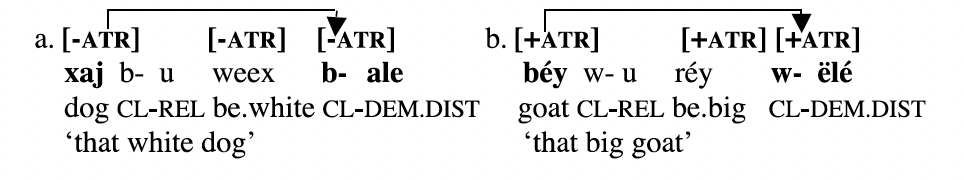
\includegraphics[scale = 0.65]{images/wolof.png}
\end{exe}
\begin{tikzpicture}[remember picture, overlay, >={Triangle[]}]
	\draw [->] (SyExatr1) |- ++(1,0.5) -| (SyExatr2);
	\draw [->] (SyExatr3) |- ++(1,0.5) -| (SyExatr4);
\end{tikzpicture}


\subsection{Irregular imperfective converb}\label{section:morphophono:auxiliary:imperfective}
All the preceding data focused on the perfective converb suffix. This suffix shows an inconstant or variable form, with or without a final liquid: [-el/ɻ] or [-e]. Whether a liquid surfaces or not is based   on the presence and location of the auxiliary. We find exactly the same behavior in another suffix: the irregular imperfective [-i(s)]. 

For regular verbs and most irregular verbs, the imperfective converb is formed by adding the suffix \textit{-um} onto the verb root or stem. In contrast, there are two irregular verbs `to give' and `to come' which form their imperfective converb  by adding the suffix \textit{-is} to the infinitive (Table \ref{tab:imperfective converb regular irregular ofrms}). Paradigms for these irregular verbs are given in \S\ref{section:verb:irregular:suppletive}.\footnote{{\seaSEA} utilizes the same irregular imperfective forms for the verbs `to come' [ɡ-ɑ-l],  `to give' [t-ɑ-l], and  `to cry' [l-ɑ-l].  But in {\iaIA},  the verb [l-ɑ-l] `to cry'   is replaced by regular [lɒt͡sʰ-e-l] `to cry' which forms its imperfective converb with \textit{-um}: [lɒt͡sʰ-um]. See \S\ref{section:verb:irregular:other} for discussion of  this verb.}

\begin{table}
	\caption{Formation of regular and irregular imperfective converbs}
	\label{tab:imperfective converb regular irregular ofrms}
% 	\resizebox{\textwidth}{!}{%
		\begin{tabular}{l ll lll}
			\lsptoprule
			& \multicolumn{2}{c}{Regular} &  \multicolumn{3}{c}{Irregular} \\\cmidrule(lr){2-3}\cmidrule(lr){4-6}
			&  \multicolumn{2}{l}{`to sing'} &  `to give' &  \multicolumn{2}{l}{`to come'} \\\midrule
			\textsc{inf} & jeɻkʰ-e-l &  $\sqrt{}$-{\thgloss}-{\infgloss}& t-ɒ-l & ɡ-ɒ-l &  $\sqrt{}$-{\thgloss}-{\infgloss}\\
			& \armenian{երգել} & & \armenian{տալ} & \armenian{գալ} & \\\addlinespace
			{\impfcvb} & jeɻkʰ-um&  $\sqrt{}$-{\impfcvb} & t-ɒ-l-is & ɡ-ɒ-l-is &  $\sqrt{}$-{\thgloss}-{\infgloss}-{\impfcvb}\\
			& \armenian{երգում} & & \armenian{տալիս} & \armenian{գալիս} & \\
			\lspbottomrule
		\end{tabular}%
% 	}
\end{table}


In \S\ref{section:morphophono:auxiliary:syntax}, we saw that the regular suffix \textit{-um} has a constant form and never alternates. In contrast,  the  irregular suffix  surfaces  as \textit{-is}   before the auxiliary, and as \textit{-i} when the auxiliary has shifted leftwards (\ref{sent:MorphoPhono:Liqid:IrrgImpf:ex}). 



\begin{exe}
	\ex \label{sent:MorphoPhono:Liqid:IrrgImpf:ex}
	\begin{xlist}
		\ex \gll jes  ɡiɻkʰ-ə  \uline{\textbf{t-ɒ-l-is}}  \colorbox{lsLightGray}{=e-m}
		\\
		I  book-{\defgloss}  give-{\thgloss}-{\infgloss}-{\impfcvb}  ={\auxgloss}-1{\sg}
		\\
		\trans `I am giving the book.' \hfill (NK)
		\\
		\armenian{Ես գիրքը տալիս եմ։}  
		\ex \gll jes  ɡiɻkʰ-ə \textbf{t͡ʃʰ\colorbox{lsLightGray}{-e-m}}  \uline{{t-ɒ-l-i}}  
		\\
		I  book-{\defgloss}    {\neggloss}={\auxgloss}-1{\sg} give-{\thgloss}-{\infgloss}-{\impfcvb}
		\\
		\trans `I am not giving  the book.' \hfill (NK)
		\\
		\armenian{Ես գիրքը չեմ  տալի։}
		\ex \gll jes  \textbf{ɡiɻkʰ} \colorbox{lsLightGray}{=e-m}  \uline{{t-ɒ-l-i}}  
		\\
		I  book    ={\auxgloss}-1{\sg} give-{\thgloss}-{\infgloss}-{\impfcvb}
		\\
		\trans `I am giving  books.'   \hfill (NK)
		\\
		\armenian{Ես գիրք եմ տալի։}
		\ex \gll \textbf{jes} \colorbox{lsLightGray}{=e-m}  ɡiɻkʰ-ə     \uline{{t-ɒ-l-i}}  
		\\
		I  {\auxgloss}-1{\sg} book-{\defgloss}   give-{\thgloss}-{\infgloss}-{\impfcvb}
		\\
		\trans `\textbf{\uline{I}} am  giving  the book.' \hfill (NK)
		\\
		\armenian{Ես եմ գիրքը   տալի։}
	\end{xlist}
\end{exe}

The imperfective [-is]$\sim$[-i] alternation happens in the same contexts as the perfective [-el/ɻ]$\sim$[-e] alternation. 	We report additional data from AS's work (\ref{sent:MorphoPhono:Liqid:IrrgImpf:AS}). The same generalization stands: if the auxiliary has shifted leftwards, then the suffix [-is] alternates with [-i].

\begin{exe}
	\ex\label{sent:MorphoPhono:Liqid:IrrgImpf:AS}
	\begin{xlist}
		\ex \gll \textbf{uʃ}  \colorbox{lsLightGray}{=e-n}   \uline{ɡ-ɒ-l-i}
		\\
		late ={\auxgloss}-3{\pl} come-{\thgloss}-{\infgloss}-{\impfcvb} 
		\\
		\trans `They are coming late.' \hfill (AS)
		\\
		\armenian{Ուշ են գալի։}
		\ex \gll \textbf{mez}  \colorbox{lsLightGray}{=e-n}   \uline{t-ɒ-l-i}
		\\
		us.{\dat} ={\auxgloss}-3{\pl} give-{\thgloss}-{\infgloss}-{\impfcvb} 
		\\
		\trans `They are giving it to us.' \hfill (AS)
		\\
		\armenian{Մեզ են տալի։}
		\ex \gll jes d͡zez-i \textbf{χoskʰ}  \colorbox{lsLightGray}{=e-m}   \uline{t-ɒ-l-i} voɻ ɒχt͡ʃʰik-əs el jeɻpʰekʰ sent͡sʰ bɒn-er t͡ʃʰ-i-$\emptyset$ ɒn-e-l-u
		\\
		I you.{\pl}-{\dat} promise ={\auxgloss}-3{\pl} give-{\thgloss}-{\infgloss}-{\impfcvb} that daughter-{\possFsg}  ever never these thing-{\pl} {\neggloss}-{\auxgloss}-3{\sg} do{\thgloss}-{\infgloss}-{\futcvb}
		\\
		\trans `I promise you that my daughter will never do these things.'  \hfill (AS)
		\\
		\armenian{Ես ձեզի խօսք եմ տալի որ աղջիկս էլ երբէք սենց բաներ չի անելու։} 
	\end{xlist}
\end{exe}




We likewise see the same long-distance conditions in reduced coordination (\ref{sent:MorphoPhono:Liqid:IrrgImpf:Coord}). The suffix surfaces as [-is] when the auxiliary is to the right within the phrase, even if not adjacent to the suffix. The suffix surfaces as [-i] when the auxiliary shifts leftwards.\largerpage


\begin{exe}
	\ex \label{sent:MorphoPhono:Liqid:IrrgImpf:Coord}
	\begin{xlist}
		\ex \gll \uline{{t-ɒ-l-is}} \colorbox{lsLightGray}{=e-m} kɒm \uline{{t͡sɒχ-um}} \colorbox{lsLightGray}{=e-m} \\
		give-{\thgloss}-{\infgloss}-{\impfcvb} ={\auxgloss}-1{\sg} or sell-{\impfcvb} ={\auxgloss}-1{\sg}
		\\
		\trans `I am giving or I am selling.' \hfill (NK)
		\\
		\armenian{Տալիս եմ կամ ծախում եմ։}
		\ex \gll \uline{{t-ɒ-l-is}}        kɒm \uline{{t͡sɒχ-um}} \colorbox{lsLightGray}{=e-m} \\
		give-{\thgloss}-{\infgloss}-{\impfcvb}     or sell-{\impfcvb} ={\auxgloss}-1{\sg}
		\\
		\trans `I am giving or selling.' \hfill (NK)
		\\
		\armenian{Տալիս  կամ ծախում եմ։}
  \ex \gll \textbf{t͡ʃʰ\colorbox{lsLightGray}{-e-m}} \uline{{t-ɒ-l-i}}        kɒm \uline{{t͡sɒχ-um}}  \\
		{\neggloss}={\auxgloss}-1{\sg} give-{\thgloss}-{\infgloss}-{\impfcvb}     or sell-{\impfcvb} 
		\\
		\trans `I am not giving or selling.' \hfill (NK)
		\\
		\armenian{Չեմ տալի   կամ ծախում ։}
\end{xlist}	\end{exe}




\subsection{Diachronic origins and effects of adjacency}\label{section:morphophono:auxiliary:EA}\largerpage

The previous section examined the synchronic behavior of the perfective converb suffix \textit{-el/eɻ} and how this suffix loses its liquid when the auxiliary has shifted. This section  describes the diachronic origins of this behavior in Standard and {\seaCEA}. 



In {\seaSEA}, the perfective converb suffix is \textit{-el}, and   the irregular imperfective converb suffix is \textit{-is}. Whereas these suffixes alternate in {\iaIA}, they do not  in {\seaSE} (\ref{sent:MorphoPhono:Liqid:History:sea}). The forms of the suffixes remain constant regardless of whether the auxiliary has shifted leftwards. 

\begin{exe}
	\ex Constant forms in {\seaSEA}\label{sent:MorphoPhono:Liqid:History:sea}
	\begin{xlist}
		\ex \gll \textbf{\uline{ɡəɾ-el}} \colorbox{lsLightGray}{=e-m}, \textbf{\uline{t-ɑ-l-is}} \colorbox{lsLightGray}{=e-m}
		\\
		write-{\perfcvb} ={\auxgloss}-1{\sg}, give-{\thgloss}-{\infgloss}-{\impfcvb} ={\auxgloss}-1{\sg}
		\\
		\trans `I have written, I am giving.'
		\\
		\armenian{Գրել եմ, տալիս եմ։}
		\ex \gll \textbf{t͡ʃʰ\colorbox{lsLightGray}{-e-m}} \uline{ɡəɾ-el}, \textbf{t͡ʃʰ\colorbox{lsLightGray}{-e-m}} \uline{t-ɑ-l-is}  
		\\
		{\neggloss}={\auxgloss}-1{\sg} write-{\perfcvb}, {\neggloss}={\auxgloss}-1{\sg} give-{\thgloss}-{\infgloss}-{\impfcvb}  
		\\
		\trans `I have not written, I am not giving.'
		\\
		\armenian{Չեմ գրել, չեմ  տալիս։}
	\end{xlist}
\end{exe}

\begin{sloppypar}
The {\iaIA} suffix [-el/-eɻ] developed from the  same historical source as the  {\seaSE} suffix. It is reported that across Armenian lects, the liquid of the perfective suffix    can sometimes change from /l/ to a rhotic (\citealt{grigoryan-2018-FallOfLiquidLPastParticipleInversionSpokenLanguage}; dialectological feature \#85 in \citealt[101]{Jahukyan-1972-ArmenianDiaolectology}). 
\end{sloppypar}

However, in {\seaCEA} (\seaCEAAbbre)  as spoken in Yerevan, it is reported that speakers can optionally drop the liquid /l/ and the fricative /s/ when the auxiliary has shifted (\ref{sent:MorphoPhono:Liqid:History:cea}) (\citealt[101]{Gharagyulyan-1981-ColloquialArmenian}, \citealt[213, 223]{DumTragut-2009-ArmenianReferenceGrammar}, \citealt[37]{KhamoyanEtAl-2014-ColloquialYerevanLanguage}).\pagebreak


\begin{exe}
	\ex Optional deletion in {\seaCEA}\label{sent:MorphoPhono:Liqid:History:cea}
	\begin{xlist}
		\ex \gll \textbf{\uline{ɡəɾ-el}} \colorbox{lsLightGray}{=e-m}, \textbf{\uline{t-ɑ-l-is}} \colorbox{lsLightGray}{=e-m}
		\\
		write-{\perfcvb} ={\auxgloss}-1{\sg}, give-{\thgloss}-{\infgloss}-{\impfcvb} ={\auxgloss}-1{\sg}
		\\
		\trans `I have written, I am giving.'
		\\
		\armenian{Գրել եմ, տալիս եմ։}
		\ex \gll \textbf{t͡ʃʰ\colorbox{lsLightGray}{-e-m}} \uline{ɡəɾ-e(l)}, \textbf{t͡ʃʰ\colorbox{lsLightGray}{-e-m}} \uline{t-ɑ-l-i(s)}  
		\\
		{\neggloss}={\auxgloss}-1{\sg} write-{\perfcvb}, {\neggloss}={\auxgloss}-1{\sg} give-{\thgloss}-{\infgloss}-{\impfcvb}  
		\\
		\trans `I have not written, I am not giving.'
		\\
		\armenian{Չեմ գրել, չեմ  տալիս։}
	\end{xlist}
\end{exe}

The deletion of the final liquid   is reported to be unique to the perfective converb suffix  [-el] in {\seaCEA}. This colloquial process is likewise attested in the {\seaCEA}   spoken by immigrant communities in Los Angeles  \citep[72]{Karapetian-2014-TeachArmenianEasternArmenianHeritage}. 


There is some experimental evidence   that this optional deletion process in {\seaCEA} is related to   the prosodic weakening of liquids \citep{grigoryan-2018-FallOfLiquidLPastParticipleInversionSpokenLanguage}.  


One speaker of {\seaCEAAbbre} (VP)    informed us that the clitic [=el] `also, even' can also optionally delete its liquid in {\seaCEAAbbre} (\ref{sent:MorphoPhono:Liqid:History:ceaOther}). 

\begin{exe}
	\ex {\seaCEA}\\ \gll jes e(l) kʰez =e-m spɑs-um 
	\\
	I also you.{\sg}.{\dat} ={\auxgloss}-1{\sg} wait-{\impfcvb}
	\\
	\trans `I am also waiting for you.' \hfill (VP) \label{sent:MorphoPhono:Liqid:History:ceaOther}
	\\
	\armenian{Ես էլ քեզ եմ սպասում։}
\end{exe}


For {\seaCEA}, we  asked young speakers from Armenia (around 20--40 years old) for their sociolinguistic intuitions about the optional deletion in the suffixes [-el] and [-is] (Table \ref{tab:coll ea judgment people}). Some speakers told us that they themselves have this optional process in their speech, some told us they do not do it at all. Some told us that this process is common, while others told us that it is judged as “vulgar” and uncommon. Some told us that they can apply the deletion in some verbs, but not others.\largerpage

\vfill
\begin{table}[H]
	\caption{Consultants on {\seaCEA} and their meta-linguistic judgments\label{tab:coll ea judgment people}}
	\resizebox{\textwidth}{!}{%
		\begin{tabular}{lllll}
			\lsptoprule
			Speaker& Age& Sex & What verbs? & Social judgment? \\\midrule
			MA & late-20s & F &   `open', `close', `eat', `drink' & ``it's colloquial''\\
			VP & mid-30s & M & any verb & ``any social class/region''\\
			HH & early-20s & M & N/A & ``it's colloquial and vulgar''\\ 
			\lspbottomrule
		\end{tabular}
	}
\end{table}
\vfill\pagebreak

The above reports suggest that this colloquial process is attested but stigmatized. The use of this process varies by speaker, and sometimes by   verb. There is little to no work on the variationist sociolinguistics of Armenian,\footnote{To our knowledge, the closest work is Zakaryan  \citep{Zakaryan-1981-ColloquialArmenian}, a study of social factors in different Armenian morphophonological choices.}   so we do not know if any demographic factors are correlated with this deletion process.



Diachronically,  there is an obvious path of historical development for the perfective suffix in {\iaIA}. 1) In some stage of the dialect, there was no deletion at all  [-el] (like modern {\seaSEA}). 2) Later on, the dialect developed optional deletion [-e(l)] (like modern  {\seaCEA}). 3)   Finally, the deletion became obligatory [-e] (as in modern {\iaIA}).  As we   discuss below, stages 2 (for {\seaCEAAbbre}) and 3 (for {\iaAbbre}) also seem to differ in terms of adjacency requirements between the suffix and the auxiliary. 

%{\added}


		Data on this colloquial process is sparse, but we suspect that {\seaCE} and {\iaIA} differ in the role of adjacency between the verb and auxiliary. Briefly, in {\iaIA}, non-adjacent auxiliaries cause the liquid to surface, while non-adjacent auxiliaries can cause the liquid to delete. We illustrate below. 

Consider the sentences in (\ref{colloq coordination el base unreduced reduced}), in both {\seaCE} and   {\iaIA}. In (\ref{colloq coordination el base unreduced reduced: unreduced}), the sentence has un-reduced coordination with two verbs and two auxiliaries. The verb's liquid surfaces in both dialects. But in   reduced coordination (\ref{colloq coordination el base unreduced reduced: reduced}) with just one auxiliary, Verb1 keeps its liquid in {\iaIA} but can optionally delete it in {\seaCEA}. No deletion is found in {\seaSE}. We use -\textsc{p}, ={\auxgloss} instead of -{\perfcvb}, ={\auxgloss}-1{\sg}.\largerpage[-2]

\begin{exe}
	\ex Effect of verb-auxiliary adjacency in {\seaCE} and   {\iaIA}\label{colloq coordination el base unreduced reduced}
	
	\begin{xlist}
		\ex Un-reduced coordination with two auxiliaries\label{colloq coordination el base unreduced reduced: unreduced}\\
		\begin{tabular}{@{}l llllll l@{}}
			& Verb1 & Aux  & Conj & Verb2 & Aux 
			\\
			i. & \uline{χəm-el} & \colorbox{lsLightGray}{=e-m}& kɑm & \uline{keɾ-el} & \colorbox{lsLightGray}{=e-m} & ({\seaAbbre})  & (MA, VP)\\
			
			ii. & \uline{χəm-el} &\colorbox{lsLightGray}{=e-m}& kɑm & \uline{keɾ-el} &\colorbox{lsLightGray}{=e-m} & ({\seaCEAAbbre}) &  (MA, VP)   \\
			& \multicolumn{5}{l}{\armenian{Խմել եմ կամ կերել եմ։}}  & 
			\\
			iii. & \uline{χəm-eɻ} & \colorbox{lsLightGray}{=e-m}& kɒm & \uline{keɻ-eɻ} & \colorbox{lsLightGray}{=e-m}& ({\iaAbbre}) & (NK)\\
			& drink-\textsc{p} & ={\auxgloss} & or & eat-\textsc{p}& ={\auxgloss} & 
			\\
			& \multicolumn{5}{l}{`I have drunk or have eaten.'}  & 
			\\
			& \multicolumn{5}{l}{\armenian{Խմեր եմ կամ կերեր եմ։}}  & 
		\end{tabular}
		\pagebreak\ex Reduced coordination with one auxiliary\label{colloq coordination el base unreduced reduced: reduced}\\
		\begin{tabular}{@{}l llllll l@{}}
			& Verb1 &   & Conj & Verb2 & Aux
			\\
			i. & \uline{χəm-el} & ~~~~~~~~~~~          & kɑm & \uline{keɾ-el} & \colorbox{lsLightGray}{=e-m} & ({\seaAbbre})  &  (MA, VP) \\
			ii. & \uline{χəm-e(l)} &\ & kɑm & \uline{keɾ-el} &\colorbox{lsLightGray}{=e-m} & ({\seaCEAAbbre})  & (MA, VP) \\
			& \multicolumn{5}{l}{\armenian{Խմել  կամ կերել եմ։}}  & 
			\\
			
			iii. & \uline{χəm-eɻ} & & kɒm & \uline{keɻ-eɻ} & \colorbox{lsLightGray}{=e-m}& ({\iaAbbre}) & (NK)	\\
			& drink-\textsc{p} &   & or & eat-\textsc{p}& ={\auxgloss} & 
			\\
			& \multicolumn{5}{l}{`I have drunk or   eaten.'}  & 
			\\
			& \multicolumn{5}{l}{\armenian{Խմեր  կամ կերեր եմ։}}  & 
		\end{tabular}
		
	\end{xlist}
\end{exe}




When reduced coordination is negated, {\seaSE} keeps the liquid in Verb1, while   {\iaIA} deletes the liquids in both Verb1 and Verb2 (\ref{ex:morphophono:liq:diach:ceanegkam}). For {\seaCEA}, either both liquids surface or both delete. Other permutations are not possible for our informants (liquid + no liquid, no liquid + liquid). 



\begin{exe}
	\ex Reduced coordination with negation and consonant-initial conjunction\label{ex:morphophono:liq:diach:ceanegkam}\\	
	\begin{tabular}{l llllll l}
		& Neg-Aux & Verb1 &     Conj & Verb2 &
		\\
		i. & \textbf{t͡ʃʰ\colorbox{lsLightGray}{-e-m}}&  \uline{χəm-el}         & kɑm & \uline{keɾ-el}  & ({\seaAbbre})  & (MA, VP) \\
		ii. & \textbf{t͡ʃʰ\colorbox{lsLightGray}{-e-m}}& \uline{χəm-el}    & kɑm & \uline{keɾ-el}   & ({\seaCEAAbbre}) &  (MA, VP) \\
		& \textbf{t͡ʃʰ\colorbox{lsLightGray}{-e-m}}& \uline{χəm-e}    & kɑm & \uline{keɾ-e}   &  & (MA, VP) \\
		& *\textbf{t͡ʃʰ\colorbox{lsLightGray}{-e-m}}& \uline{χəm-e}    & kɑm & \uline{keɾ-el}   &  & (*MA, *VP) \\
		& *\textbf{t͡ʃʰ\colorbox{lsLightGray}{-e-m}}& \uline{χəm-el}    & kɑm & \uline{keɾ-e}   &  & (*MA, *VP) \\
		& \multicolumn{5}{l}{\armenian{Չեմ խմել  կամ կերել։}}  & 
		\\
		
		iii. & \textbf{t͡ʃʰ\colorbox{lsLightGray}{-e-m}}& \uline{χəm-e} &  kɒm & \uline{keɻ-e}  & ({\iaAbbre}) & (NK)	\\
		& {\neggloss}={\auxgloss}& drink-\textsc{p} &     or & eat-\textsc{p} & 
		\\
		& \multicolumn{5}{l}{`I have not drunk or   eaten.'}  & 
		\\
		& \multicolumn{5}{l}{\armenian{Չեմ խմէ կամ կերէ։}} & 
	\end{tabular}
	
\end{exe}






The generalization so far is the following. In both {\iaIA} and {\seaCEA}, the auxiliary licenses the floating liquid of the perfective converb. In {\iaIA}, the suffix and auxiliary do not need to be adjacent, but they do need to be adjacent in {\seaCEA}.% We can formalize this variation with the following rules, adapted from Rule \ref{fig:docking perf v2}. 
%
%\begin{ruleblock}
%	{\textbf{Liquid retention}: Dialect variation for the morpheme-specific rule of anchoring (surfacing) floating segments before the auxiliary}
%	\label{fig:docking perf v2 eas}
%	
%	\begin{center}
%		\begin{tabular}{|llll|llll|  }
%			\hline 
%			\multicolumn{4}{| l| }{{\iaAbbre} } & \multicolumn{4}{| l| }{{\seaCEAAbbre} }
%			\\
%			\multicolumn{4}{| l| }{Non-adjacent conditioning } & \multicolumn{4}{| l| }{Adjacent conditioning}
%			\\
%			
%			$<$C$>$ & $\rightarrow$  & C & / [ \_ $\dots$ {\auxgloss} ]
%			& 
%			$<$C$>$ & $\rightarrow$  & C & / [ \_   {\auxgloss} ]
%			\\
%			\hline 
%			
%		\end{tabular}
%		
%	\end{center}	
%\end{ruleblock}

The above generalization  is however too simplified for   {\seaCEA}, because we have found some variation across speakers. In reduced coordination with a vowel-initial conjunction, one {\seaSE} speaker  told us that they can delete the liquid on Verb1 (VP), while another said that they could not (MA). This data suggests that some speakers can allow other adjacent vowel-initial words to license the perfective liquid (\ref{ex:morphophono:liq:diach:ceaVword}). 



\begin{exe}
	\ex Effect of other vowel-initial words   in {\seaCEA} and in {\iaIA}\label{ex:morphophono:liq:diach:ceaVword}
	
	\begin{xlist}
		\ex Un-reduced coordination with two auxiliaries
		
		\begin{tabular}{@{}l llllll l@{}}
			& Verb1 & Aux  & Conj & Verb2 & Aux\\
			i. & \uline{χəm-el} & \colorbox{lsLightGray}{=e-m}& u & \uline{keɾ-el} & \colorbox{lsLightGray}{=e-m} & ({\seaAbbre})  & \\
			ii. & \uline{χəm-el} &\colorbox{lsLightGray}{=e-m}& u & \uline{keɾ-el} &\colorbox{lsLightGray}{=e-m} & ({\seaCEAAbbre})  \\
			& \multicolumn{5}{l}{\armenian{Խմել եմ ու կերել եմ։}}  & 
			\\
			
			iii. & \uline{χəm-eɻ} & \colorbox{lsLightGray}{=e-m}& u & \uline{keɻ-eɻ} & \colorbox{lsLightGray}{=e-m}& ({\iaAbbre}) & (NK) 	\\
			& drink-\textsc{p} & ={\auxgloss} & and & eat-\textsc{p}& ={\auxgloss} & 
			\\
			& \multicolumn{5}{l}{`I have drunk and have eaten.'}  & 
			\\
			& \multicolumn{5}{l}{\armenian{Խմեր եմ ու կերեր եմ։}}  & 
		\end{tabular}
		\ex Reduced coordination with one auxiliary
		
		\begin{tabular}{@{}l llllll l@{}}
			& Verb1 &   & Conj & Verb2 & Aux
			\\
			i. & \uline{χəm-el} & ~~~~~~~~~~~          & u & \uline{keɾ-el} & \colorbox{lsLightGray}{=e-m} & ({\seaAbbre})  & (MA, VP) \\
			ii. & \uline{χəm-el} &\ & u & \uline{keɾ-el} &\colorbox{lsLightGray}{=e-m} & ({\seaCEAAbbre})  &  (VP, MA) \\
			& \uline{χəm-e} &\ & u & \uline{keɾ-el} &\colorbox{lsLightGray}{=e-m} & ({\seaCEAAbbre})  &  (VP, *MA)\\
			& \multicolumn{5}{l}{\armenian{Խմել  կամ կերել եմ։}}  & 
			\\
			
			iii. & \uline{χəm-eɻ} & & u & \uline{keɻ-eɻ} & \colorbox{lsLightGray}{=e-m}& ({\iaAbbre}) & (NK) 	\\
			& drink-\textsc{p} &   & and & eat-\textsc{p}& ={\auxgloss} & 
			\\
			& \multicolumn{5}{l}{`I have drunk and   eaten.'}  & 
			\\
			& \multicolumn{5}{l}{\armenian{Խմեր  ու կերեր եմ։}}  & 
		\end{tabular}
		
	\end{xlist}
\end{exe}

The variation can cause ineffability      when reduced coordination involves negation and a vowel-initial conjunction (\ref{ex:morphophono:liq:diach:ceaVConjNeg}). In the sentences below, the auxiliary has to shift because of negation, and Verb1 precedes a vowel. Our consultants VP and MA are fine with deleting neither liquid. VP is fine with deleting both  liquids, but MA is not. Neither speaker is fine with deleting only one liquid.  For {\iaIA}, our main consultant required deletion in both verbs. However, another speaker (GE) reports that deletion of the first liquid is optional. 


\begin{exe}
	\ex Reduced coordination with negation and vowel-initial conjunction\label{ex:morphophono:liq:diach:ceaVConjNeg}
	
	\begin{tabular}{l llllll l}
		& Neg-Aux & Verb1 &     Conj & Verb2 &
		\\
		i. & \textbf{t͡ʃʰ\colorbox{lsLightGray}{-e-m}}&  \uline{χəm-el}         & u & \uline{keɾ-el}  & ({\seaAbbre})  & (VP, MA) \\
		ii. & \textbf{t͡ʃʰ\colorbox{lsLightGray}{-e-m}}& \uline{χəm-el}    & u & \uline{keɾ-el}   & ({\seaCEAAbbre}) &  (VP, MA) \\
		& \textbf{t͡ʃʰ\colorbox{lsLightGray}{-e-m}}& \uline{χəm-e}    & u & \uline{keɾ-e}   &  & (VP, *MA) \\
		& *\textbf{t͡ʃʰ\colorbox{lsLightGray}{-e-m}}& \uline{χəm-e}    & u & \uline{keɾ-el}   &  & (*VP, *MA) \\
		& *\textbf{t͡ʃʰ\colorbox{lsLightGray}{-e-m}}& \uline{χəm-el}    & u & \uline{keɾ-e}   &  & (*VP, *MA) \\
		& \multicolumn{5}{l}{\armenian{Չեմ խմել  ու կերել։}}  & 
		\\
	\end{tabular}\\
	\begin{tabular}{l llllll l}
		iii. & \textbf{t͡ʃʰ\colorbox{lsLightGray}{-e-m}}& \uline{χəm-e} &  u & \uline{keɻ-e}  & ({\iaAbbre}) & (NK) 	\\
		   & \textbf{t͡ʃʰ\colorbox{lsLightGray}{-e-m}}& \uline{χəm-e(l)} &  u & \uline{keɻ-e}  & ({\iaAbbre}) & (GE) 	\\
				& {\neggloss}={\auxgloss}& drink-\textsc{p} &     and & eat-\textsc{p} & 
		\\
		& \multicolumn{5}{l}{`I have not drunk and   eaten.'}  & 
		\\
		& \multicolumn{5}{l}{\armenian{Չեմ խմէ ու կերէ։}} & 
	\end{tabular}
\end{exe}

The data from {\seaCEA} and {\iaIA} is  quite complicated and our analysis is incomplete. More variation-oriented data is required from larger pools of people from different areas and  generations.  But crucially, the overarching generalization is that whereas {\iaAbbre} allows non-local conditioning between the suffix and the auxiliary, {\seaCEAAbbre} seems to require local conditioning.   Some {\iaAbbre} speakers also allow both generalizations simultaneously (non-local or local conditioning).

